\chapter{面向动态数据可用性的纠删码对象存储策略}
\section{引言}
现有的基于纠删码的分布式文件系统,如 Hadoop 分布式文件系统、Ceph 分布式文件系统和 Tahoe-LAFS 分布式文件系统等,均需要在存储系统进行初始化时确定纠删码的编码方案,在存储系统初始化后,除非重新创建新的存储池,并不能动态地调整数据块和校验块的数量。在上一章中,我们提出了基于不同类型的存储设备的状态进行数据可用性的推断策略,在本章中,我们将继续讨论 On-demand ARECS 算法,单独对每个具有不同的可用性需求的数据对象,根据系统实时状态计算数据块和校验块的编码方案,并选取最快的存储节点集合,从而实现基于动态数据可用性定义的高效对象存储。我们还将基于 Tahoe-LAFS 分布式文件系统实现 On-demand ARECS 算法,并部署一个分布式文件系统作为测试环境,对自适应纠删码对象存储策略 On-demand ARECS 的实际性能进行评估。

对于由 $s$ 块硬盘组成的分布式存储系统,若待存储的对象持久性需求为 $p_{f}'$,对象使用纠删码的方式冗余存储于此分布式存储系统的 $n+m$ 块磁盘中,其存储方案的数据正确率为 $p_{f}(n,m)$。我们需要在能满足对象持久性需求,即满足约束 $p_{f}(n,m) \geq p_{f}'$ 的若干组纠删码方案中,寻找速度最快的一组方案完成存储操作。在本章中,我们针对所有可能的存储方案组合计算读写所需要的时间 $t_{f}(n+m)$,并选择读写时间 $t_{f}(n+m)$ 最小的磁盘组,这样选取的磁盘组便是可以满足对象持久性需求的速度最快的磁盘组。即通过动态计算 $p_{d_j}$ 和 $t_{f}(n+m)$,选取满足 $p_{f}(n,m) \geq p_{f}'$ 且 $t_{f}(n+m)$ 最小的纠删码方案,作为分布式存储系统在当前的工作状况下最优的纠删码编码方案,从而在满足对象的可用性需求的所有存储方案中,选取当前状况下存储速度最快的方案,避免了传统算法确定性编码方案的使用,更加快速地将数据存储于分布式存储系统。
\section{基于动态数据可用性的编码方案选择算法}
对于 On-demand ARECS 算法来说,需要我们首先确定数据的可用性。根据上一章的分析我们可以得知,由于边际成本较边际收益增加幅度更快,因此选取合理的对象持久性,可以最大限度的提高成本收益率。On-demand ARECS 算法需要我们根据数据本身的特征选取合适的对象持久性,对于较为重要的数据,选取较高的 $p_{f}'$,对于一般的数据,选取较低的 $p_{f}'$,在此基础上进行算法的优化选择。

其次 On-demand ARECS 算法根据磁盘的属性等信息预测磁盘的可靠性。我们通过读取磁盘的 S.M.A.R.T. 信息,获得磁盘的重分配扇区数 $N_{RS}$,并通过统计数据中心中所有磁盘中和所有损坏磁盘中 $N_{RS}$ 的分布,依靠贝叶斯定理计算当前磁盘的故障率:
$$
p_d=\dfrac{\mathrm{num.\ of\ failed\ disks\ with\ }N_{RS}}{\mathrm{num.\ of\ all\ disks\ with\ }N_{RS}}
$$

在得出对象持久性和磁盘可靠性之后,我们便可以依据对象可用性和磁盘可靠性的关系计算存储的纠删码方案,通过上一章中的分析与计算,我们可以得知编码块数 $m$ 的取值为:
$$
m(n)=\left\lceil\operatorname*{argmin}_{m}f(n,m)\right\rceil,\ \operatorname*{where}\ f(n,m) \geq 0
$$

其中 $f(n,m)$ 为:
\begin{align*}
f(n,m)=\sum_{i=0}^{m}\sum_{{\forall}S_{d}{\in}S_{a}(n+m,i)}&\left[\left(\prod_{{\forall}d_{j}{\in}S_{d}}\left(1-(1-p_{d_j})^{t_r}\right)\right)\right.\\
&\cdot\left.\left(\prod_{{\forall}d_{j}{\in}S_{d}'(n+m)-S_{d}}(1-p_{d_j})^{t_{r}}\right)\right]-p_{f}^{t_{r}}
\end{align*}

因此,我们便可以基于此选择数据冗余度最低的纠删码编码方案 $(n+m,n)$ 及其对应的磁盘组 $S_{d}'(n+m)$。需要注意的是,由于不同磁盘可能存在故障率相同的情况,且 $m$ 的选取对 $\displaystyle\operatorname*{argmin}_{m}f(n,m)$ 进行了向上取整操作,因此此处的 $S_{d}'(n+m)$ 存在不止一组满足条件的组合。
\section{基于存储速度的节点选择策略}
\subsection{单个数据块磁盘组读写时间的计算}
由于在编码方案选择的过程中选取的 $m$ 值和磁盘组 $S_{d}'(n+m)$ 依赖于 $n$ 值的确定,且对于相同的 $(n+m,n)$ 编码方案,存在多种满足条件的磁盘组合 $S_{d}'(n+m)$,因此我们需要根据存储设备当前的负载等信息,从候选磁盘组中选取速度最快的一组,作为最终存储数据的磁盘组。我们可以用磁盘当前进行一个读写操作所需要的时间,来代表存储设备的速度。在本节中,我们首先对存储系统中单个数据块的读写时间进行计算。

对于分布式文件系统中的磁盘来说,其读写时间主要由以下三部分操作所需要的事件共同组成:
\begin{itemize}
\item 队列等待时间 $t_{queue}$:当存储系统负载过大时,磁盘的读写请求不能被实时处理,操作系统便会将请求放入磁盘读写队列中依次进行调度,在读写请求发出到操作系统实际调度执行之间的等待时间便是磁盘的队列等待时间,通过优化磁盘调度算法、平衡节点读写请求等方式可以有效地降低队列等待时间
\item 读写延迟 $t_{latency}$:对于本地磁盘的读写,需要通过寻道等操作确定数据的位置,对于远程磁盘的读写,需要与远程磁盘建立连接并传输读写请求,这些操作均会产生磁盘的读写延迟,在分布式存储系统中,我们可以采用就近调度等方案来减少读写延迟
\item 数据写入时间:数据实际的写入时间仅取决于待写入的数据量 $data\_size$ 和磁盘的数据传输带宽 $bandwidth$,对于分布式文件系统,可以通过增加节点间的传输带宽来提高数据写入时间
\end{itemize}

可以看出,磁盘的总读写时间 $t_{d}$ 应为以上三个步骤所需要的时间之和,具体可以表示为:
$$
t_{d}=t_{queue}+t_{latency}+\dfrac{data\_size}{bandwidth}
$$

对于使用互联网传输的分布式存储系统来说,由于网络环境波动等原因,读写延迟和数据传输带宽是实时发生变化的。因此,我们在计算总的磁盘读写时间 $t_{d}$ 时,需要动态采集读写延时和数据传输带宽。在 On-demand ARECS 算法中,我们在存储系统中的节点每次进行数据读写时,将本次操作的读写延时和数据传输带宽等关键参数进行保存,以便存储系统后续进行写入时使用。

对于分布式存储系统来说,不同节点之间的读写操作是相对独立的,因此可以认为数据在不同节点间是并行读写的。因此,总读写时间实际上就是所有节点均完成读写所需要的时间,即所有节点的读写时间 $t_{d_i}$ 中的最大值 $\displaystyle\max_{d_{i}{\in}S_{d}'(n+m)}t_{d_i}$。对于纠删码分布式存储系统来说,在数据进行写入之前,需要首先进行纠删码校验码的编码计算,因此需要再加上纠删码编码所耗费的 CPU 时间 $t_{calc}$。进而此纠删码分布式存储系统的总读写时间可以表示为:
$$
t_{f}(n+m)=t_{calc}+\max_{d_{i}{\in}S_{d}'(n+m)}t_{d_i}
$$
\subsection{分块存储的对象所需总磁盘读写时间的计算}
对于较大的对象,为避免直接采用纠删码编码时编码矩阵过大,计算效率过低的问题,我们可以将较大的数据分为多个块,不同块之间可以并行进行存储,从而提高存储效率。若将数据分为 $r$ 块 $(b_{1},b_{2},\cdots,b_{r})$,则每一块数据的读写时间分别为:
$$
\begin{cases}
\left(t_{f}(n+m)\right)_{b_{1}}=(t_{calc})_{b_{1}}+\left(\displaystyle\max_{d_{i}{\in}S_{d}'(n+m)}t_{d_i}\right)_{b_{1}}\\
\left(t_{f}(n+m)\right)_{b_{2}}=(t_{calc})_{b_{2}}+\left(\displaystyle\max_{d_{i}{\in}S_{d}'(n+m)}t_{d_i}\right)_{b_{2}}\\
\vdots\\
\left(t_{f}(n+m)\right)_{b_{r}}=(t_{calc})_{b_{r}}+\left(\displaystyle\max_{d_{i}{\in}S_{d}'(n+m)}t_{d_i}\right)_{b_{r}}\\
\end{cases}
$$

我们不妨假设数据从 $b_{1}$ 到 $b_{r}$ 按照顺序依次传输,那么存储系统处理这些数据所用的总读写时间为:
$$
t_{f}(n+m)=\sum_{x=1}^{r}\left(t_{f}(n+m)\right)_{b_{x}}
$$

即:
$$
t_{f}(n+m)=\sum_{x=1}^{r}\left((t_{calc})_{b_{x}}+\left(\max_{d_{i}{\in}S_{d}'(n+m)}t_{d_i}\right)_{b_{x}}\right)
$$

但由于数据的计算和数据的传输可以并行执行,在传输前一个数据块的内容的同时,可以同时并行进行后一个数据块的编码计算,即传输 $b_{i}$ 和 $b_{i+1}$ 块所用的时间不是:
$$
\left(t_{f}(n+m)\right)_{\{b_{i},b_{i+1}\}}=(t_{calc})_{b_{i}}+\left(\max_{d_{i}{\in}S_{d}'(n+m)}t_{d_i}\right)_{b_{i}}+(t_{calc})_{b_{i+1}}+\left(\max_{d_{i}{\in}S_{d}'(n+m)}t_{d_i}\right)_{b_{i+1}}
$$

而应该是:
\begin{align*}
\left(t_{f}(n+m)\right)_{\{b_{i},b_{i+1}\}}&=(t_{calc})_{b_{i}}+\max\left(\left(\max_{d_{i}{\in}S_{d}'(n+m)}t_{d_i}\right)_{b_{i}},(t_{calc})_{b_{i+1}}\right)\\
&\quad+\left(\max_{d_{i}{\in}S_{d}'(n+m)}t_{d_i}\right)_{b_{i+1}}
\end{align*}

因此,传输这 $r$ 个数据块所需要花费的总时间可以表达为:
\begin{align*}
t_{f}(n+m)&=(t_{calc})_{b_1}+\left(\sum_{x=2}^{r}\max\left((t_{calc})_{b_{x-1}},\left(\max_{d_{i}{\in}S_{d}'(n+m)}t_{d_i}\right)_{b_{x}}\right)\right)\\
&\quad+\left(\max_{d_{i}{\in}S_{d}'(n+m)}t_{d_i}\right)_{b_r}
\end{align*}

由于在实际的分布式存储系统实现中,我们一般将数据切分为大小确定且均等的数据块,故对于上式来说,可以取 $(t_{calc})_{b_x}=t_{calc}$,$\left(\displaystyle\max_{d_{i}{\in}S_{d}'(n+m)}t_{d_i}\right)_{b_{x}}=\displaystyle\max_{d_{i}{\in}S_{d}'(n+m)}t_{d_i}$。因此我们可以得到实际的分布式存储系统中数据编码和传输所需要的总时间:
$$
t_{f}(n+m)=t_{calc}+\max_{d_{i}{\in}S_{d}'(n+m)}t_{d_i}+(r-1)\left(\max\left(t_{calc},\max_{d_{i}{\in}S_{d}'(n+m)}t_{d_i}\right)\right)
$$
\subsection{基于最小化磁盘读写时间的存储节点组合选择策略}
根据 Liu 等人的研究\cite{liu2018implementation},在数据量一定的的前提下,随着数据分块数 $n$ 的增大,虽然数据冗余度有所下降,但纠删码的编码时间迅速上升。因此,需要我们综合考虑数据冗余度和存储速度,选取数据分块数 $n$ 相对较小且数据冗余度不过高的编码方案,无需考虑 $n$ 值过大的存储策略所对应的存储方案,从而降低存储系统中纠删码编码所用的时间,提高存储系统的性能。

在此基础上,我们需要在所有满足上述条件的磁盘组 $S_{d}'(n+m)$ 中选取存储延时 $t_{f}(n+m)$ 最小的磁盘组,即选取的磁盘组为:
$$
S_{d}'(n+m)=\operatorname*{argmin}_{S_{d}'(n+m)}{t_{f}(n+m)}
$$

代入上一节中得到的数据均等切分情况下数据编码和传输所需要的总时间 $t_{f}(n+m)$,得到选取的磁盘组为:
$$
S_{d}'(n+m)=\operatorname*{argmin}_{S_{d}'(n+m)}\left(t_{calc}+\max_{d_{i}{\in}S_{d}'(n+m)}t_{d_i}+(r-1)\left(\max\left(t_{calc},\max_{d_{i}{\in}S_{d}'(n+m)}t_{d_i}\right)\right)\right)
$$
\section{实验与分析}
\subsection{实验环境}
为了验证 On-demand ARECS 算法动态选择纠删码编码策略和存储节点的算法效果,我们基于 Tahoe-LAFS 分布式文件系统\cite{wilcox2008tahoe}实现了 On-demand ARECS 算法。Tahoe-LAFS 是一个免费、开源、安全、去中心化、容错性好的分布式存储和分布式文件系统,其围绕“最小权限原则”(Principle of Least Authority,即 POLA)进行设计和实现,严格使用加密传输数据,并针对每项功能仅提供能完成相应操作的最小特权集。由于数据均进行了加密和冗余备份,因此存储系统中的每个节点均无需保证其可靠性。Tahoe-LAFS 的纠删码引擎基于 zfec 纠删码编码库实现,其提供了三种不同类型的节点:
\begin{itemize}
\item 介绍节点:介绍节点负责连接分布式存储系统中所有的存储节点和客户节点,作为节点间的信息传输的一个桥梁,联系起分布式文件系统的所有节点
\item 存储节点:存储节点负责实际的数据存储,由纠删码编码的原始数据块和冗余校验块均存储于存储节点
\item 客户节点:客户节点负责提供分布式文件系统的用户接口,并将用户的读写请求转换为实际存储节点的操作指令传输给存储节点
\end{itemize}

在 Tahoe-LAFS 分布式文件系统的默认纠删码引擎配置中,针对所有数据均采用 $(n+m,n)=(10,3)$ 的纠删码编码策略。Tahoe-LAFS 分布式文件系统将文件先进行加密,然后分为若干数据单元,每个单元独立进行编码。Tahoe-LAFS 分布式文件系统将每个单元的数据切分为 $n$ 个原始数据块,并通过纠删码编码矩阵计算得出 $m$ 个冗余校验块。之后,Tahoe-LAFS 分布式文件系统随机选取 $n+m$ 个剩余存储空间足够的存储节点,并将这 $n+m$ 个块分别存储于这些存储节点中。

我们在 Tahoe-LAFS 分布式文件系统的基础上实现了 On-demand ARECS 算法,从而动态地确定纠删码编码策略和存储节点。我们在基于 KVM 虚拟化技术的分布式集群中,部署了一个由 37 个节点组成的分布式文件系统实验环境,具体信息如表 \ref{t2} 和图 \ref{p6} 所示。存储系统中一共有 3 种不同的节点:客户节点、A 类存储节点和 B 类存储节点。客户节点共有 1 个,充当 Tahoe-LAFS 分布式文件系统中的客户节点和介绍节点,负责进行实验操作,发出存储请求并进行测试。A 类存储节点为资源相对受限的存储节点,其计算资源、存储资源和存储可靠性均相对较低。B 类存储节点为相对优质的存储节点,其计算资源、存储资源和存储可靠性均相对较高。所有的存储节点平均分为三组,每组各有 6 个 A 类存储节点和 6 个 B 类存储节点。三组存储节点和客户节点分别放置在不同的机房中。

\begin{table}[!htb]
\centering
\caption{不同存储节点的配置}
\begin{tabular}{c|c|c}
\hline
存储节点种类 & Storage Server A & Storage Server B\\\hline
vCPU 数量 & 1 vCPU & 2 vCPU\\\hline
内存容量 & 1 GB & 2 GB\\\hline
磁盘容量 & 25 GB & 60 GB\\\hline
磁盘的故障率 $p_{d}$ & 8.6\% & 1.7\%\\\hline
\end{tabular}
\label{t2}
\end{table}

为了避免机房由于不可抗力的原因发生数据丢失,我们采用异地备份的方法,将三个存储节点的集群分别布置于荷兰阿姆斯特丹(以下简称 AMS)、德国法兰克福(以下简称 FRA)和英国伦敦(以下简称 LON),将客户节点布置于美国纽约(以下简称 NYC),这可以最大限度地满足在 On-demand ARECS 模型中的对磁盘损坏事件独立性的假设。由于 On-demand ARECS 算法考虑了到不同节点间的网络波动问题,因此我们使用真实的国际互联网在节点之间传输数据,以期得到更贴近于实际应用的实验数据。我们在实验过程中对各机房之间的平均通讯延迟(Round-Trip Time,即 RTT)和平均带宽的进行了多次测量,其平均值如图 \ref{p6} 所示。由于在国际互联网中不同机房间链路的拥挤程度不同,节点间的平均通讯延迟与节点间的数据传输带宽并不完全成负相关关系。在网络不发生拥堵的情况下,节点间的平均通讯延迟主要取决于节点间的地理距离,而节点间的数据传输带宽主要取决于节点间光缆的建设容量。即使两个节点相距较远,由于光速的限制无法达到较低的通讯延迟,仍可以通过增大网络容量等方式达到较大的传输带宽。比如图 \ref{p6} 中 LON 节点到 FRA 节点的平均通讯延迟高于其到 AMS 节点的平均通讯延迟,但测得的数据传输带宽则是 LON 节点到 FRA 节点更高。

\begin{figure}[!htb]
\centering
\resizebox{.8\textwidth}{!}{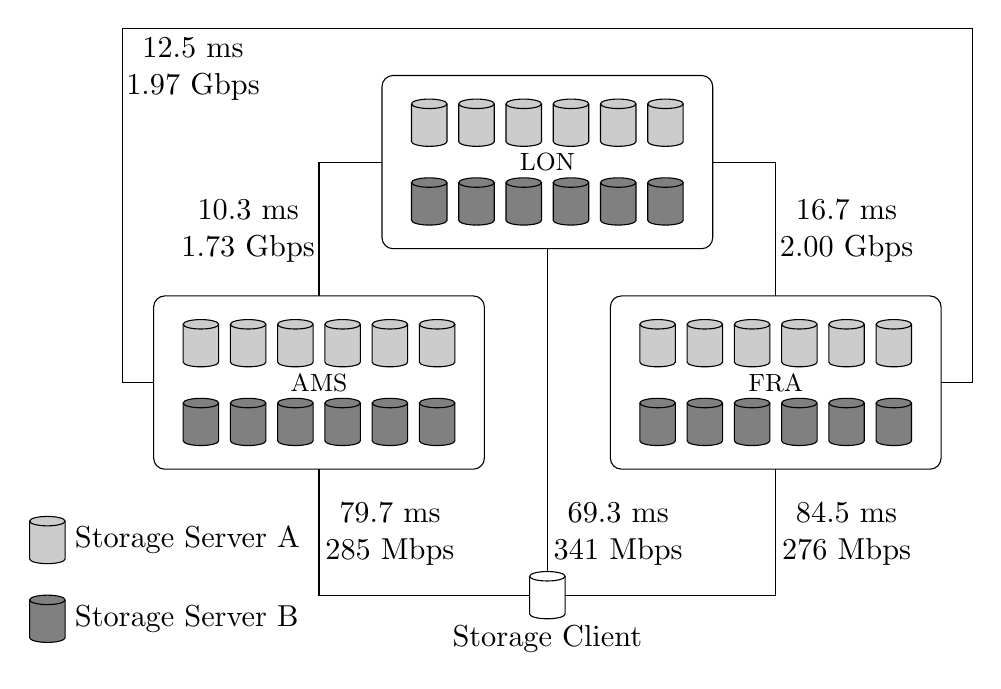
\begin{tikzpicture}
\newcommand\cylinderwidth{.75}
\newcommand\cylinder[3]{%
\draw (#2, #3+.8*#1) ellipse (\cylinderwidth*#1 and .2*#1);%
\draw (#2-\cylinderwidth*#1, #3+.8*#1) -- (#2-\cylinderwidth*#1, #3-.8*#1) arc (180:360:\cylinderwidth*#1 and .2*#1) -- (#2+\cylinderwidth*#1, #3+.8*#1);%
}
\newcommand\cylinderA[3]{%
\fill [color=black!20!white] (#2-\cylinderwidth*#1, #3-.8*#1) arc (180:360:\cylinderwidth*#1 and .2*#1) -- (#2+\cylinderwidth*#1, #3+.8*#1) arc (0:180:\cylinderwidth*#1 and .2*#1) -- cycle;%
\cylinder{#1}{#2}{#3}%
}
\newcommand\cylinderB[3]{%
\fill [color=black!50!white] (#2-\cylinderwidth*#1, #3-.8*#1) arc (180:360:\cylinderwidth*#1 and .2*#1) -- (#2+\cylinderwidth*#1, #3+.8*#1) arc (0:180:\cylinderwidth*#1 and .2*#1) -- cycle;%
\cylinder{#1}{#2}{#3}%
}
\newcommand\cluster[3]{%
\draw [rounded corners] (#1-2.1, #2-1.1) rectangle (#1+2.1, #2+1.1);%
\node at (#1, #2) [font=\fontsize{9pt}{20pt}\selectfont] {#3};%
\cylinderA{.3}{#1-1.5}{#2+.5}%
\cylinderA{.3}{#1-.9}{#2+.5}%
\cylinderA{.3}{#1-.3}{#2+.5}%
\cylinderA{.3}{#1+.3}{#2+.5}%
\cylinderA{.3}{#1+.9}{#2+.5}%
\cylinderA{.3}{#1+1.5}{#2+.5}%
\cylinderB{.3}{#1-1.5}{#2-.5}%
\cylinderB{.3}{#1-.9}{#2-.5}%
\cylinderB{.3}{#1-.3}{#2-.5}%
\cylinderB{.3}{#1+.3}{#2-.5}%
\cylinderB{.3}{#1+.9}{#2-.5}%
\cylinderB{.3}{#1+1.5}{#2-.5}%
}
\fill [color=white,opacity=0] (0, 0) rectangle (12, 8);

\cluster{6.6}{6.3}{LON}
\cluster{9.5}{3.5}{FRA}
\cluster{3.7}{3.5}{AMS}
\cylinder{.3}{6.6}{.8}
\node at (6.6, .25) [font=\fontsize{10.5pt}{20pt}\selectfont] {Storage Client};

\draw (1.6, 3.5) -- (1.2, 3.5) -- (1.2, 8) -- (12, 8) -- (12, 3.5) -- (11.6, 3.5);
\draw (3.7, 4.6) -- (3.7, 6.3) -- (4.5, 6.3);
\draw (9.5, 4.6) -- (9.5, 6.3) -- (8.7, 6.3);

\draw (6.6-.3*\cylinderwidth, .8) -- (3.7, .8) -- (3.7, 2.4);
\draw (6.6+.3*\cylinderwidth, .8) -- (9.5, .8) -- (9.5, 2.4);
\draw (6.6, 1.1) -- (6.6, 5.2);

\cylinderA{.3}{.25}{1.5}
\node at (2.1, 1.5) [font=\fontsize{10.5pt}{20pt}\selectfont] {\hbox to 3cm{Storage Server A\hss}};
\cylinderB{.3}{.25}{.5}
\node at (2.1, .5) [font=\fontsize{10.5pt}{20pt}\selectfont] {\hbox to 3cm{Storage Server B\hss}};

\node at (2.1, 7.75) [font=\fontsize{10.5pt}{20pt}\selectfont] {12.5 ms};
\node at (2.1, 7.25) [font=\fontsize{10.5pt}{20pt}\selectfont] {1.97 Gbps};

\node at (2.8, 5.7) [font=\fontsize{10.5pt}{20pt}\selectfont] {10.3 ms};
\node at (2.8, 5.2) [font=\fontsize{10.5pt}{20pt}\selectfont] {1.73 Gbps};

\node at (10.4, 5.7) [font=\fontsize{10.5pt}{20pt}\selectfont] {16.7 ms};
\node at (10.4, 5.2) [font=\fontsize{10.5pt}{20pt}\selectfont] {2.00 Gbps};

\node at (7.5, 1.85) [font=\fontsize{10.5pt}{20pt}\selectfont] {69.3 ms};
\node at (7.5, 1.35) [font=\fontsize{10.5pt}{20pt}\selectfont] {341 Mbps};

\node at (10.4, 1.85) [font=\fontsize{10.5pt}{20pt}\selectfont] {84.5 ms};
\node at (10.4, 1.35) [font=\fontsize{10.5pt}{20pt}\selectfont] {276 Mbps};

\node at (4.6, 1.85) [font=\fontsize{10.5pt}{20pt}\selectfont] {79.7 ms};
\node at (4.6, 1.35) [font=\fontsize{10.5pt}{20pt}\selectfont] {285 Mbps};
\end{tikzpicture}
}
\caption{Tahoe-LAFS 实验集群示意}
\label{p6}
\end{figure}
\subsection{实验结果与分析}
在上述实验环境中,我们使用随机生成的实验方法,创建了三种不同的测试数据对象文件,其大小分别为 10 MB、50 MB 和 200 MB。在实验系统中,我们分别针对这三种数据对象测试了 On-demand ARECS 算法的存储速度,得到了在不同分块情况 $(n+m,n)$ 下的文件传输时间如图 \ref{p7} 所示。

\begin{figure}[!htb]
\centering
\resizebox{.8\textwidth}{!}{%% Creator: Matplotlib, PGF backend
%%
%% To include the figure in your LaTeX document, write
%%   \input{<filename>.pgf}
%%
%% Make sure the required packages are loaded in your preamble
%%   \usepackage{pgf}
%%
%% Figures using additional raster images can only be included by \input if
%% they are in the same directory as the main LaTeX file. For loading figures
%% from other directories you can use the `import` package
%%   \usepackage{import}
%% and then include the figures with
%%   \import{<path to file>}{<filename>.pgf}
%%
%% Matplotlib used the following preamble
%%   \usepackage{xeCJK}
%%   \setCJKmainfont{SimSun}
%%   \usepackage{fontspec}
%%
\begingroup%
\makeatletter%
\begin{pgfpicture}%
\pgfpathrectangle{\pgfpointorigin}{\pgfqpoint{6.400000in}{4.800000in}}%
\pgfusepath{use as bounding box, clip}%
\begin{pgfscope}%
\pgfsetbuttcap%
\pgfsetmiterjoin%
\definecolor{currentfill}{rgb}{1.000000,1.000000,1.000000}%
\pgfsetfillcolor{currentfill}%
\pgfsetlinewidth{0.000000pt}%
\definecolor{currentstroke}{rgb}{1.000000,1.000000,1.000000}%
\pgfsetstrokecolor{currentstroke}%
\pgfsetdash{}{0pt}%
\pgfpathmoveto{\pgfqpoint{0.000000in}{0.000000in}}%
\pgfpathlineto{\pgfqpoint{6.400000in}{0.000000in}}%
\pgfpathlineto{\pgfqpoint{6.400000in}{4.800000in}}%
\pgfpathlineto{\pgfqpoint{0.000000in}{4.800000in}}%
\pgfpathclose%
\pgfusepath{fill}%
\end{pgfscope}%
\begin{pgfscope}%
\pgfsetbuttcap%
\pgfsetmiterjoin%
\definecolor{currentfill}{rgb}{1.000000,1.000000,1.000000}%
\pgfsetfillcolor{currentfill}%
\pgfsetlinewidth{0.000000pt}%
\definecolor{currentstroke}{rgb}{0.000000,0.000000,0.000000}%
\pgfsetstrokecolor{currentstroke}%
\pgfsetstrokeopacity{0.000000}%
\pgfsetdash{}{0pt}%
\pgfpathmoveto{\pgfqpoint{0.800000in}{0.528000in}}%
\pgfpathlineto{\pgfqpoint{5.760000in}{0.528000in}}%
\pgfpathlineto{\pgfqpoint{5.760000in}{4.224000in}}%
\pgfpathlineto{\pgfqpoint{0.800000in}{4.224000in}}%
\pgfpathclose%
\pgfusepath{fill}%
\end{pgfscope}%
\begin{pgfscope}%
\pgfsetbuttcap%
\pgfsetroundjoin%
\definecolor{currentfill}{rgb}{0.000000,0.000000,0.000000}%
\pgfsetfillcolor{currentfill}%
\pgfsetlinewidth{0.803000pt}%
\definecolor{currentstroke}{rgb}{0.000000,0.000000,0.000000}%
\pgfsetstrokecolor{currentstroke}%
\pgfsetdash{}{0pt}%
\pgfsys@defobject{currentmarker}{\pgfqpoint{0.000000in}{-0.048611in}}{\pgfqpoint{0.000000in}{0.000000in}}{%
\pgfpathmoveto{\pgfqpoint{0.000000in}{0.000000in}}%
\pgfpathlineto{\pgfqpoint{0.000000in}{-0.048611in}}%
\pgfusepath{stroke,fill}%
}%
\begin{pgfscope}%
\pgfsys@transformshift{0.869969in}{0.528000in}%
\pgfsys@useobject{currentmarker}{}%
\end{pgfscope}%
\end{pgfscope}%
\begin{pgfscope}%
\pgftext[x=0.869969in,y=0.430778in,,top]{\rmfamily\fontsize{14.000000}{16.800000}\selectfont 0}%
\end{pgfscope}%
\begin{pgfscope}%
\pgfsetbuttcap%
\pgfsetroundjoin%
\definecolor{currentfill}{rgb}{0.000000,0.000000,0.000000}%
\pgfsetfillcolor{currentfill}%
\pgfsetlinewidth{0.803000pt}%
\definecolor{currentstroke}{rgb}{0.000000,0.000000,0.000000}%
\pgfsetstrokecolor{currentstroke}%
\pgfsetdash{}{0pt}%
\pgfsys@defobject{currentmarker}{\pgfqpoint{0.000000in}{-0.048611in}}{\pgfqpoint{0.000000in}{0.000000in}}{%
\pgfpathmoveto{\pgfqpoint{0.000000in}{0.000000in}}%
\pgfpathlineto{\pgfqpoint{0.000000in}{-0.048611in}}%
\pgfusepath{stroke,fill}%
}%
\begin{pgfscope}%
\pgfsys@transformshift{1.647398in}{0.528000in}%
\pgfsys@useobject{currentmarker}{}%
\end{pgfscope}%
\end{pgfscope}%
\begin{pgfscope}%
\pgftext[x=1.647398in,y=0.430778in,,top]{\rmfamily\fontsize{14.000000}{16.800000}\selectfont 5}%
\end{pgfscope}%
\begin{pgfscope}%
\pgfsetbuttcap%
\pgfsetroundjoin%
\definecolor{currentfill}{rgb}{0.000000,0.000000,0.000000}%
\pgfsetfillcolor{currentfill}%
\pgfsetlinewidth{0.803000pt}%
\definecolor{currentstroke}{rgb}{0.000000,0.000000,0.000000}%
\pgfsetstrokecolor{currentstroke}%
\pgfsetdash{}{0pt}%
\pgfsys@defobject{currentmarker}{\pgfqpoint{0.000000in}{-0.048611in}}{\pgfqpoint{0.000000in}{0.000000in}}{%
\pgfpathmoveto{\pgfqpoint{0.000000in}{0.000000in}}%
\pgfpathlineto{\pgfqpoint{0.000000in}{-0.048611in}}%
\pgfusepath{stroke,fill}%
}%
\begin{pgfscope}%
\pgfsys@transformshift{2.424828in}{0.528000in}%
\pgfsys@useobject{currentmarker}{}%
\end{pgfscope}%
\end{pgfscope}%
\begin{pgfscope}%
\pgftext[x=2.424828in,y=0.430778in,,top]{\rmfamily\fontsize{14.000000}{16.800000}\selectfont 10}%
\end{pgfscope}%
\begin{pgfscope}%
\pgfsetbuttcap%
\pgfsetroundjoin%
\definecolor{currentfill}{rgb}{0.000000,0.000000,0.000000}%
\pgfsetfillcolor{currentfill}%
\pgfsetlinewidth{0.803000pt}%
\definecolor{currentstroke}{rgb}{0.000000,0.000000,0.000000}%
\pgfsetstrokecolor{currentstroke}%
\pgfsetdash{}{0pt}%
\pgfsys@defobject{currentmarker}{\pgfqpoint{0.000000in}{-0.048611in}}{\pgfqpoint{0.000000in}{0.000000in}}{%
\pgfpathmoveto{\pgfqpoint{0.000000in}{0.000000in}}%
\pgfpathlineto{\pgfqpoint{0.000000in}{-0.048611in}}%
\pgfusepath{stroke,fill}%
}%
\begin{pgfscope}%
\pgfsys@transformshift{3.202257in}{0.528000in}%
\pgfsys@useobject{currentmarker}{}%
\end{pgfscope}%
\end{pgfscope}%
\begin{pgfscope}%
\pgftext[x=3.202257in,y=0.430778in,,top]{\rmfamily\fontsize{14.000000}{16.800000}\selectfont 15}%
\end{pgfscope}%
\begin{pgfscope}%
\pgfsetbuttcap%
\pgfsetroundjoin%
\definecolor{currentfill}{rgb}{0.000000,0.000000,0.000000}%
\pgfsetfillcolor{currentfill}%
\pgfsetlinewidth{0.803000pt}%
\definecolor{currentstroke}{rgb}{0.000000,0.000000,0.000000}%
\pgfsetstrokecolor{currentstroke}%
\pgfsetdash{}{0pt}%
\pgfsys@defobject{currentmarker}{\pgfqpoint{0.000000in}{-0.048611in}}{\pgfqpoint{0.000000in}{0.000000in}}{%
\pgfpathmoveto{\pgfqpoint{0.000000in}{0.000000in}}%
\pgfpathlineto{\pgfqpoint{0.000000in}{-0.048611in}}%
\pgfusepath{stroke,fill}%
}%
\begin{pgfscope}%
\pgfsys@transformshift{3.979687in}{0.528000in}%
\pgfsys@useobject{currentmarker}{}%
\end{pgfscope}%
\end{pgfscope}%
\begin{pgfscope}%
\pgftext[x=3.979687in,y=0.430778in,,top]{\rmfamily\fontsize{14.000000}{16.800000}\selectfont 20}%
\end{pgfscope}%
\begin{pgfscope}%
\pgfsetbuttcap%
\pgfsetroundjoin%
\definecolor{currentfill}{rgb}{0.000000,0.000000,0.000000}%
\pgfsetfillcolor{currentfill}%
\pgfsetlinewidth{0.803000pt}%
\definecolor{currentstroke}{rgb}{0.000000,0.000000,0.000000}%
\pgfsetstrokecolor{currentstroke}%
\pgfsetdash{}{0pt}%
\pgfsys@defobject{currentmarker}{\pgfqpoint{0.000000in}{-0.048611in}}{\pgfqpoint{0.000000in}{0.000000in}}{%
\pgfpathmoveto{\pgfqpoint{0.000000in}{0.000000in}}%
\pgfpathlineto{\pgfqpoint{0.000000in}{-0.048611in}}%
\pgfusepath{stroke,fill}%
}%
\begin{pgfscope}%
\pgfsys@transformshift{4.757116in}{0.528000in}%
\pgfsys@useobject{currentmarker}{}%
\end{pgfscope}%
\end{pgfscope}%
\begin{pgfscope}%
\pgftext[x=4.757116in,y=0.430778in,,top]{\rmfamily\fontsize{14.000000}{16.800000}\selectfont 25}%
\end{pgfscope}%
\begin{pgfscope}%
\pgfsetbuttcap%
\pgfsetroundjoin%
\definecolor{currentfill}{rgb}{0.000000,0.000000,0.000000}%
\pgfsetfillcolor{currentfill}%
\pgfsetlinewidth{0.803000pt}%
\definecolor{currentstroke}{rgb}{0.000000,0.000000,0.000000}%
\pgfsetstrokecolor{currentstroke}%
\pgfsetdash{}{0pt}%
\pgfsys@defobject{currentmarker}{\pgfqpoint{0.000000in}{-0.048611in}}{\pgfqpoint{0.000000in}{0.000000in}}{%
\pgfpathmoveto{\pgfqpoint{0.000000in}{0.000000in}}%
\pgfpathlineto{\pgfqpoint{0.000000in}{-0.048611in}}%
\pgfusepath{stroke,fill}%
}%
\begin{pgfscope}%
\pgfsys@transformshift{5.534545in}{0.528000in}%
\pgfsys@useobject{currentmarker}{}%
\end{pgfscope}%
\end{pgfscope}%
\begin{pgfscope}%
\pgftext[x=5.534545in,y=0.430778in,,top]{\rmfamily\fontsize{14.000000}{16.800000}\selectfont 30}%
\end{pgfscope}%
\begin{pgfscope}%
\pgftext[x=3.280000in,y=0.202556in,,top]{\rmfamily\fontsize{14.000000}{16.800000}\selectfont 数据分块数 \(\displaystyle n\)}%
\end{pgfscope}%
\begin{pgfscope}%
\pgfsetbuttcap%
\pgfsetroundjoin%
\definecolor{currentfill}{rgb}{0.000000,0.000000,0.000000}%
\pgfsetfillcolor{currentfill}%
\pgfsetlinewidth{0.803000pt}%
\definecolor{currentstroke}{rgb}{0.000000,0.000000,0.000000}%
\pgfsetstrokecolor{currentstroke}%
\pgfsetdash{}{0pt}%
\pgfsys@defobject{currentmarker}{\pgfqpoint{-0.048611in}{0.000000in}}{\pgfqpoint{0.000000in}{0.000000in}}{%
\pgfpathmoveto{\pgfqpoint{0.000000in}{0.000000in}}%
\pgfpathlineto{\pgfqpoint{-0.048611in}{0.000000in}}%
\pgfusepath{stroke,fill}%
}%
\begin{pgfscope}%
\pgfsys@transformshift{0.800000in}{0.611196in}%
\pgfsys@useobject{currentmarker}{}%
\end{pgfscope}%
\end{pgfscope}%
\begin{pgfscope}%
\pgftext[x=0.607500in,y=0.543723in,left,base]{\rmfamily\fontsize{14.000000}{16.800000}\selectfont 0}%
\end{pgfscope}%
\begin{pgfscope}%
\pgfsetbuttcap%
\pgfsetroundjoin%
\definecolor{currentfill}{rgb}{0.000000,0.000000,0.000000}%
\pgfsetfillcolor{currentfill}%
\pgfsetlinewidth{0.803000pt}%
\definecolor{currentstroke}{rgb}{0.000000,0.000000,0.000000}%
\pgfsetstrokecolor{currentstroke}%
\pgfsetdash{}{0pt}%
\pgfsys@defobject{currentmarker}{\pgfqpoint{-0.048611in}{0.000000in}}{\pgfqpoint{0.000000in}{0.000000in}}{%
\pgfpathmoveto{\pgfqpoint{0.000000in}{0.000000in}}%
\pgfpathlineto{\pgfqpoint{-0.048611in}{0.000000in}}%
\pgfusepath{stroke,fill}%
}%
\begin{pgfscope}%
\pgfsys@transformshift{0.800000in}{1.158179in}%
\pgfsys@useobject{currentmarker}{}%
\end{pgfscope}%
\end{pgfscope}%
\begin{pgfscope}%
\pgftext[x=0.512222in,y=1.090707in,left,base]{\rmfamily\fontsize{14.000000}{16.800000}\selectfont 50}%
\end{pgfscope}%
\begin{pgfscope}%
\pgfsetbuttcap%
\pgfsetroundjoin%
\definecolor{currentfill}{rgb}{0.000000,0.000000,0.000000}%
\pgfsetfillcolor{currentfill}%
\pgfsetlinewidth{0.803000pt}%
\definecolor{currentstroke}{rgb}{0.000000,0.000000,0.000000}%
\pgfsetstrokecolor{currentstroke}%
\pgfsetdash{}{0pt}%
\pgfsys@defobject{currentmarker}{\pgfqpoint{-0.048611in}{0.000000in}}{\pgfqpoint{0.000000in}{0.000000in}}{%
\pgfpathmoveto{\pgfqpoint{0.000000in}{0.000000in}}%
\pgfpathlineto{\pgfqpoint{-0.048611in}{0.000000in}}%
\pgfusepath{stroke,fill}%
}%
\begin{pgfscope}%
\pgfsys@transformshift{0.800000in}{1.705163in}%
\pgfsys@useobject{currentmarker}{}%
\end{pgfscope}%
\end{pgfscope}%
\begin{pgfscope}%
\pgftext[x=0.416944in,y=1.637691in,left,base]{\rmfamily\fontsize{14.000000}{16.800000}\selectfont 100}%
\end{pgfscope}%
\begin{pgfscope}%
\pgfsetbuttcap%
\pgfsetroundjoin%
\definecolor{currentfill}{rgb}{0.000000,0.000000,0.000000}%
\pgfsetfillcolor{currentfill}%
\pgfsetlinewidth{0.803000pt}%
\definecolor{currentstroke}{rgb}{0.000000,0.000000,0.000000}%
\pgfsetstrokecolor{currentstroke}%
\pgfsetdash{}{0pt}%
\pgfsys@defobject{currentmarker}{\pgfqpoint{-0.048611in}{0.000000in}}{\pgfqpoint{0.000000in}{0.000000in}}{%
\pgfpathmoveto{\pgfqpoint{0.000000in}{0.000000in}}%
\pgfpathlineto{\pgfqpoint{-0.048611in}{0.000000in}}%
\pgfusepath{stroke,fill}%
}%
\begin{pgfscope}%
\pgfsys@transformshift{0.800000in}{2.252147in}%
\pgfsys@useobject{currentmarker}{}%
\end{pgfscope}%
\end{pgfscope}%
\begin{pgfscope}%
\pgftext[x=0.416944in,y=2.184674in,left,base]{\rmfamily\fontsize{14.000000}{16.800000}\selectfont 150}%
\end{pgfscope}%
\begin{pgfscope}%
\pgfsetbuttcap%
\pgfsetroundjoin%
\definecolor{currentfill}{rgb}{0.000000,0.000000,0.000000}%
\pgfsetfillcolor{currentfill}%
\pgfsetlinewidth{0.803000pt}%
\definecolor{currentstroke}{rgb}{0.000000,0.000000,0.000000}%
\pgfsetstrokecolor{currentstroke}%
\pgfsetdash{}{0pt}%
\pgfsys@defobject{currentmarker}{\pgfqpoint{-0.048611in}{0.000000in}}{\pgfqpoint{0.000000in}{0.000000in}}{%
\pgfpathmoveto{\pgfqpoint{0.000000in}{0.000000in}}%
\pgfpathlineto{\pgfqpoint{-0.048611in}{0.000000in}}%
\pgfusepath{stroke,fill}%
}%
\begin{pgfscope}%
\pgfsys@transformshift{0.800000in}{2.799130in}%
\pgfsys@useobject{currentmarker}{}%
\end{pgfscope}%
\end{pgfscope}%
\begin{pgfscope}%
\pgftext[x=0.416944in,y=2.731658in,left,base]{\rmfamily\fontsize{14.000000}{16.800000}\selectfont 200}%
\end{pgfscope}%
\begin{pgfscope}%
\pgfsetbuttcap%
\pgfsetroundjoin%
\definecolor{currentfill}{rgb}{0.000000,0.000000,0.000000}%
\pgfsetfillcolor{currentfill}%
\pgfsetlinewidth{0.803000pt}%
\definecolor{currentstroke}{rgb}{0.000000,0.000000,0.000000}%
\pgfsetstrokecolor{currentstroke}%
\pgfsetdash{}{0pt}%
\pgfsys@defobject{currentmarker}{\pgfqpoint{-0.048611in}{0.000000in}}{\pgfqpoint{0.000000in}{0.000000in}}{%
\pgfpathmoveto{\pgfqpoint{0.000000in}{0.000000in}}%
\pgfpathlineto{\pgfqpoint{-0.048611in}{0.000000in}}%
\pgfusepath{stroke,fill}%
}%
\begin{pgfscope}%
\pgfsys@transformshift{0.800000in}{3.346114in}%
\pgfsys@useobject{currentmarker}{}%
\end{pgfscope}%
\end{pgfscope}%
\begin{pgfscope}%
\pgftext[x=0.416944in,y=3.278642in,left,base]{\rmfamily\fontsize{14.000000}{16.800000}\selectfont 250}%
\end{pgfscope}%
\begin{pgfscope}%
\pgfsetbuttcap%
\pgfsetroundjoin%
\definecolor{currentfill}{rgb}{0.000000,0.000000,0.000000}%
\pgfsetfillcolor{currentfill}%
\pgfsetlinewidth{0.803000pt}%
\definecolor{currentstroke}{rgb}{0.000000,0.000000,0.000000}%
\pgfsetstrokecolor{currentstroke}%
\pgfsetdash{}{0pt}%
\pgfsys@defobject{currentmarker}{\pgfqpoint{-0.048611in}{0.000000in}}{\pgfqpoint{0.000000in}{0.000000in}}{%
\pgfpathmoveto{\pgfqpoint{0.000000in}{0.000000in}}%
\pgfpathlineto{\pgfqpoint{-0.048611in}{0.000000in}}%
\pgfusepath{stroke,fill}%
}%
\begin{pgfscope}%
\pgfsys@transformshift{0.800000in}{3.893097in}%
\pgfsys@useobject{currentmarker}{}%
\end{pgfscope}%
\end{pgfscope}%
\begin{pgfscope}%
\pgftext[x=0.416944in,y=3.825625in,left,base]{\rmfamily\fontsize{14.000000}{16.800000}\selectfont 300}%
\end{pgfscope}%
\begin{pgfscope}%
\pgftext[x=0.361389in,y=2.376000in,,bottom,rotate=90.000000]{\rmfamily\fontsize{14.000000}{16.800000}\selectfont 时间(秒)}%
\end{pgfscope}%
\begin{pgfscope}%
\pgfpathrectangle{\pgfqpoint{0.800000in}{0.528000in}}{\pgfqpoint{4.960000in}{3.696000in}}%
\pgfusepath{clip}%
\pgfsetrectcap%
\pgfsetroundjoin%
\pgfsetlinewidth{1.505625pt}%
\definecolor{currentstroke}{rgb}{0.000000,0.000000,0.000000}%
\pgfsetstrokecolor{currentstroke}%
\pgfsetdash{}{0pt}%
\pgfpathmoveto{\pgfqpoint{1.025455in}{0.811895in}}%
\pgfpathlineto{\pgfqpoint{1.180940in}{0.738818in}}%
\pgfpathlineto{\pgfqpoint{1.336426in}{0.735755in}}%
\pgfpathlineto{\pgfqpoint{1.491912in}{0.737275in}}%
\pgfpathlineto{\pgfqpoint{1.647398in}{0.739288in}}%
\pgfpathlineto{\pgfqpoint{1.802884in}{0.725482in}}%
\pgfpathlineto{\pgfqpoint{1.958370in}{0.725636in}}%
\pgfpathlineto{\pgfqpoint{2.113856in}{0.704708in}}%
\pgfpathlineto{\pgfqpoint{2.269342in}{0.707279in}}%
\pgfpathlineto{\pgfqpoint{2.424828in}{0.705725in}}%
\pgfpathlineto{\pgfqpoint{2.580313in}{0.698089in}}%
\pgfpathlineto{\pgfqpoint{2.735799in}{0.696000in}}%
\pgfpathlineto{\pgfqpoint{2.891285in}{0.701481in}}%
\pgfpathlineto{\pgfqpoint{3.046771in}{0.699205in}}%
\pgfpathlineto{\pgfqpoint{3.202257in}{0.699643in}}%
\pgfpathlineto{\pgfqpoint{3.357743in}{0.696711in}}%
\pgfpathlineto{\pgfqpoint{3.513229in}{0.700354in}}%
\pgfpathlineto{\pgfqpoint{3.668715in}{0.700299in}}%
\pgfpathlineto{\pgfqpoint{3.824201in}{0.702564in}}%
\pgfpathlineto{\pgfqpoint{3.979687in}{0.705605in}}%
\pgfpathlineto{\pgfqpoint{4.135172in}{0.706229in}}%
\pgfpathlineto{\pgfqpoint{4.290658in}{0.723743in}}%
\pgfpathlineto{\pgfqpoint{4.446144in}{0.717879in}}%
\pgfpathlineto{\pgfqpoint{4.601630in}{0.712978in}}%
\pgfpathlineto{\pgfqpoint{4.757116in}{0.712191in}}%
\pgfpathlineto{\pgfqpoint{4.912602in}{0.739627in}}%
\pgfpathlineto{\pgfqpoint{5.068088in}{0.723743in}}%
\pgfpathlineto{\pgfqpoint{5.223574in}{0.724290in}}%
\pgfpathlineto{\pgfqpoint{5.379060in}{0.727955in}}%
\pgfpathlineto{\pgfqpoint{5.534545in}{0.731138in}}%
\pgfusepath{stroke}%
\end{pgfscope}%
\begin{pgfscope}%
\pgfpathrectangle{\pgfqpoint{0.800000in}{0.528000in}}{\pgfqpoint{4.960000in}{3.696000in}}%
\pgfusepath{clip}%
\pgfsetbuttcap%
\pgfsetroundjoin%
\pgfsetlinewidth{1.505625pt}%
\definecolor{currentstroke}{rgb}{0.000000,0.000000,0.000000}%
\pgfsetstrokecolor{currentstroke}%
\pgfsetdash{{9.600000pt}{2.400000pt}{1.500000pt}{2.400000pt}}{0.000000pt}%
\pgfpathmoveto{\pgfqpoint{1.025455in}{1.463932in}}%
\pgfpathlineto{\pgfqpoint{1.180940in}{1.130097in}}%
\pgfpathlineto{\pgfqpoint{1.336426in}{1.107200in}}%
\pgfpathlineto{\pgfqpoint{1.491912in}{1.093537in}}%
\pgfpathlineto{\pgfqpoint{1.647398in}{1.041355in}}%
\pgfpathlineto{\pgfqpoint{1.802884in}{1.024595in}}%
\pgfpathlineto{\pgfqpoint{1.958370in}{1.024814in}}%
\pgfpathlineto{\pgfqpoint{2.113856in}{0.919837in}}%
\pgfpathlineto{\pgfqpoint{2.269342in}{0.912299in}}%
\pgfpathlineto{\pgfqpoint{2.424828in}{0.930951in}}%
\pgfpathlineto{\pgfqpoint{2.580313in}{0.868978in}}%
\pgfpathlineto{\pgfqpoint{2.735799in}{0.879644in}}%
\pgfpathlineto{\pgfqpoint{2.891285in}{0.876603in}}%
\pgfpathlineto{\pgfqpoint{3.046771in}{0.893910in}}%
\pgfpathlineto{\pgfqpoint{3.202257in}{0.864033in}}%
\pgfpathlineto{\pgfqpoint{3.357743in}{0.837319in}}%
\pgfpathlineto{\pgfqpoint{3.513229in}{0.848685in}}%
\pgfpathlineto{\pgfqpoint{3.668715in}{0.847132in}}%
\pgfpathlineto{\pgfqpoint{3.824201in}{0.851190in}}%
\pgfpathlineto{\pgfqpoint{3.979687in}{0.863869in}}%
\pgfpathlineto{\pgfqpoint{4.135172in}{0.881088in}}%
\pgfpathlineto{\pgfqpoint{4.290658in}{0.930164in}}%
\pgfpathlineto{\pgfqpoint{4.446144in}{0.937001in}}%
\pgfpathlineto{\pgfqpoint{4.601630in}{0.926039in}}%
\pgfpathlineto{\pgfqpoint{4.757116in}{0.917692in}}%
\pgfpathlineto{\pgfqpoint{4.912602in}{0.929168in}}%
\pgfpathlineto{\pgfqpoint{5.068088in}{0.931422in}}%
\pgfpathlineto{\pgfqpoint{5.223574in}{1.043346in}}%
\pgfpathlineto{\pgfqpoint{5.379060in}{0.960138in}}%
\pgfpathlineto{\pgfqpoint{5.534545in}{0.960346in}}%
\pgfusepath{stroke}%
\end{pgfscope}%
\begin{pgfscope}%
\pgfpathrectangle{\pgfqpoint{0.800000in}{0.528000in}}{\pgfqpoint{4.960000in}{3.696000in}}%
\pgfusepath{clip}%
\pgfsetbuttcap%
\pgfsetroundjoin%
\pgfsetlinewidth{1.505625pt}%
\definecolor{currentstroke}{rgb}{0.000000,0.000000,0.000000}%
\pgfsetstrokecolor{currentstroke}%
\pgfsetdash{{5.550000pt}{2.400000pt}}{0.000000pt}%
\pgfpathmoveto{\pgfqpoint{1.025455in}{4.056000in}}%
\pgfpathlineto{\pgfqpoint{1.180940in}{2.561192in}}%
\pgfpathlineto{\pgfqpoint{1.336426in}{2.269705in}}%
\pgfpathlineto{\pgfqpoint{1.491912in}{2.279627in}}%
\pgfpathlineto{\pgfqpoint{1.647398in}{2.226373in}}%
\pgfpathlineto{\pgfqpoint{1.802884in}{2.180295in}}%
\pgfpathlineto{\pgfqpoint{1.958370in}{2.153022in}}%
\pgfpathlineto{\pgfqpoint{2.113856in}{1.738671in}}%
\pgfpathlineto{\pgfqpoint{2.269342in}{1.740990in}}%
\pgfpathlineto{\pgfqpoint{2.424828in}{1.771129in}}%
\pgfpathlineto{\pgfqpoint{2.580313in}{1.568483in}}%
\pgfpathlineto{\pgfqpoint{2.735799in}{1.539886in}}%
\pgfpathlineto{\pgfqpoint{2.891285in}{1.547850in}}%
\pgfpathlineto{\pgfqpoint{3.046771in}{1.433181in}}%
\pgfpathlineto{\pgfqpoint{3.202257in}{1.439821in}}%
\pgfpathlineto{\pgfqpoint{3.357743in}{1.406433in}}%
\pgfpathlineto{\pgfqpoint{3.513229in}{1.406860in}}%
\pgfpathlineto{\pgfqpoint{3.668715in}{1.456985in}}%
\pgfpathlineto{\pgfqpoint{3.824201in}{1.431671in}}%
\pgfpathlineto{\pgfqpoint{3.979687in}{1.466623in}}%
\pgfpathlineto{\pgfqpoint{4.135172in}{1.527535in}}%
\pgfpathlineto{\pgfqpoint{4.290658in}{1.564719in}}%
\pgfpathlineto{\pgfqpoint{4.446144in}{1.588973in}}%
\pgfpathlineto{\pgfqpoint{4.601630in}{1.692571in}}%
\pgfpathlineto{\pgfqpoint{4.757116in}{1.654906in}}%
\pgfpathlineto{\pgfqpoint{4.912602in}{1.852586in}}%
\pgfpathlineto{\pgfqpoint{5.068088in}{1.814942in}}%
\pgfpathlineto{\pgfqpoint{5.223574in}{1.728683in}}%
\pgfpathlineto{\pgfqpoint{5.379060in}{1.819854in}}%
\pgfpathlineto{\pgfqpoint{5.534545in}{1.861633in}}%
\pgfusepath{stroke}%
\end{pgfscope}%
\begin{pgfscope}%
\pgfsetrectcap%
\pgfsetmiterjoin%
\pgfsetlinewidth{0.803000pt}%
\definecolor{currentstroke}{rgb}{0.000000,0.000000,0.000000}%
\pgfsetstrokecolor{currentstroke}%
\pgfsetdash{}{0pt}%
\pgfpathmoveto{\pgfqpoint{0.800000in}{0.528000in}}%
\pgfpathlineto{\pgfqpoint{0.800000in}{4.224000in}}%
\pgfusepath{stroke}%
\end{pgfscope}%
\begin{pgfscope}%
\pgfsetrectcap%
\pgfsetmiterjoin%
\pgfsetlinewidth{0.803000pt}%
\definecolor{currentstroke}{rgb}{0.000000,0.000000,0.000000}%
\pgfsetstrokecolor{currentstroke}%
\pgfsetdash{}{0pt}%
\pgfpathmoveto{\pgfqpoint{5.760000in}{0.528000in}}%
\pgfpathlineto{\pgfqpoint{5.760000in}{4.224000in}}%
\pgfusepath{stroke}%
\end{pgfscope}%
\begin{pgfscope}%
\pgfsetrectcap%
\pgfsetmiterjoin%
\pgfsetlinewidth{0.803000pt}%
\definecolor{currentstroke}{rgb}{0.000000,0.000000,0.000000}%
\pgfsetstrokecolor{currentstroke}%
\pgfsetdash{}{0pt}%
\pgfpathmoveto{\pgfqpoint{0.800000in}{0.528000in}}%
\pgfpathlineto{\pgfqpoint{5.760000in}{0.528000in}}%
\pgfusepath{stroke}%
\end{pgfscope}%
\begin{pgfscope}%
\pgfsetrectcap%
\pgfsetmiterjoin%
\pgfsetlinewidth{0.803000pt}%
\definecolor{currentstroke}{rgb}{0.000000,0.000000,0.000000}%
\pgfsetstrokecolor{currentstroke}%
\pgfsetdash{}{0pt}%
\pgfpathmoveto{\pgfqpoint{0.800000in}{4.224000in}}%
\pgfpathlineto{\pgfqpoint{5.760000in}{4.224000in}}%
\pgfusepath{stroke}%
\end{pgfscope}%
\begin{pgfscope}%
\pgfsetbuttcap%
\pgfsetmiterjoin%
\definecolor{currentfill}{rgb}{1.000000,1.000000,1.000000}%
\pgfsetfillcolor{currentfill}%
\pgfsetfillopacity{0.800000}%
\pgfsetlinewidth{1.003750pt}%
\definecolor{currentstroke}{rgb}{0.800000,0.800000,0.800000}%
\pgfsetstrokecolor{currentstroke}%
\pgfsetstrokeopacity{0.800000}%
\pgfsetdash{}{0pt}%
\pgfpathmoveto{\pgfqpoint{4.343278in}{3.255278in}}%
\pgfpathlineto{\pgfqpoint{5.623889in}{3.255278in}}%
\pgfpathquadraticcurveto{\pgfqpoint{5.662778in}{3.255278in}}{\pgfqpoint{5.662778in}{3.294167in}}%
\pgfpathlineto{\pgfqpoint{5.662778in}{4.087889in}}%
\pgfpathquadraticcurveto{\pgfqpoint{5.662778in}{4.126778in}}{\pgfqpoint{5.623889in}{4.126778in}}%
\pgfpathlineto{\pgfqpoint{4.343278in}{4.126778in}}%
\pgfpathquadraticcurveto{\pgfqpoint{4.304389in}{4.126778in}}{\pgfqpoint{4.304389in}{4.087889in}}%
\pgfpathlineto{\pgfqpoint{4.304389in}{3.294167in}}%
\pgfpathquadraticcurveto{\pgfqpoint{4.304389in}{3.255278in}}{\pgfqpoint{4.343278in}{3.255278in}}%
\pgfpathclose%
\pgfusepath{stroke,fill}%
\end{pgfscope}%
\begin{pgfscope}%
\pgfsetrectcap%
\pgfsetroundjoin%
\pgfsetlinewidth{1.505625pt}%
\definecolor{currentstroke}{rgb}{0.000000,0.000000,0.000000}%
\pgfsetstrokecolor{currentstroke}%
\pgfsetdash{}{0pt}%
\pgfpathmoveto{\pgfqpoint{4.382167in}{3.980944in}}%
\pgfpathlineto{\pgfqpoint{4.771056in}{3.980944in}}%
\pgfusepath{stroke}%
\end{pgfscope}%
\begin{pgfscope}%
\pgftext[x=4.926611in,y=3.912889in,left,base]{\rmfamily\fontsize{14.000000}{16.800000}\selectfont 10 MB}%
\end{pgfscope}%
\begin{pgfscope}%
\pgfsetbuttcap%
\pgfsetroundjoin%
\pgfsetlinewidth{1.505625pt}%
\definecolor{currentstroke}{rgb}{0.000000,0.000000,0.000000}%
\pgfsetstrokecolor{currentstroke}%
\pgfsetdash{{9.600000pt}{2.400000pt}{1.500000pt}{2.400000pt}}{0.000000pt}%
\pgfpathmoveto{\pgfqpoint{4.382167in}{3.709889in}}%
\pgfpathlineto{\pgfqpoint{4.771056in}{3.709889in}}%
\pgfusepath{stroke}%
\end{pgfscope}%
\begin{pgfscope}%
\pgftext[x=4.926611in,y=3.641833in,left,base]{\rmfamily\fontsize{14.000000}{16.800000}\selectfont 50 MB}%
\end{pgfscope}%
\begin{pgfscope}%
\pgfsetbuttcap%
\pgfsetroundjoin%
\pgfsetlinewidth{1.505625pt}%
\definecolor{currentstroke}{rgb}{0.000000,0.000000,0.000000}%
\pgfsetstrokecolor{currentstroke}%
\pgfsetdash{{5.550000pt}{2.400000pt}}{0.000000pt}%
\pgfpathmoveto{\pgfqpoint{4.382167in}{3.438834in}}%
\pgfpathlineto{\pgfqpoint{4.771056in}{3.438834in}}%
\pgfusepath{stroke}%
\end{pgfscope}%
\begin{pgfscope}%
\pgftext[x=4.926611in,y=3.370778in,left,base]{\rmfamily\fontsize{14.000000}{16.800000}\selectfont 200 MB}%
\end{pgfscope}%
\end{pgfpicture}%
\makeatother%
\endgroup%
}
\caption{不同数据分块数的存储时间表现}
\label{p7}
\end{figure}

分析图 \ref{p7} 我们可以看出,当数据切分数 $n$ 较小时,数据冗余度较高,因此需要传输的总数据量 $data\_size$ 更大,从而使得总文件传输时间更长。当数据切分数 $n$ 过大时,由于纠删码的编码矩阵更加复杂,编码时间 $t_{calc}$ 时间更长,同时过多的切分数需要选择更多的节点,因此选择到慢速节点的可能性更大,即数据读写延迟 $t_{calc}$ 更大,数据传输带宽 $bandwidth$ 更小,同样使得文件传输时间更长。针对本文中选取的测试环境来说,在数据切分数 $n$ 取 $n=16$ 左右时存储系统的耗时最短。故若根据实际的传输情况选择数据切分数合适的编码方案,可以很大程度上降低存储系统的文件传输时间。

在 On-demand ARECS 算法中,我们通过动态地选取最优的编码方案和数据存储节点,从而减小数据的存储延时。我们在实现了 On-demand ARECS 算法的 Tahoe-LAFS 分布式文件系统中,分别测试了原始的多备份方案以及基于 On-demand ARECS 算法的里德-所罗门码纠删码编码方案,针对上述生成的 10 MB、50 MB 和 200 MB 大小的测试数据对象文件进行了实验,实验结果如图 \ref{p8} 所示。在实验中,分析存储系统的记录可以得到,其中 On-demand ARECS 算法选取了 $(n+m,n)=(20,16)$ 的纠删码编码策略,使用的存储节点占全部存储节点的 $56\%$。原始的纠删码算法则选取了 $(n+m,n)=(10,3)$ 的纠删码编码策略,使用的存储节点占全部存储节点的 $28\%$。多副本备份方案则直接存储了 $4$ 份原始数据作为冗余备份。

\begin{figure}[!htb]
\centering
\resizebox{.8\textwidth}{!}{%% Creator: Matplotlib, PGF backend
%%
%% To include the figure in your LaTeX document, write
%%   \input{<filename>.pgf}
%%
%% Make sure the required packages are loaded in your preamble
%%   \usepackage{pgf}
%%
%% Figures using additional raster images can only be included by \input if
%% they are in the same directory as the main LaTeX file. For loading figures
%% from other directories you can use the `import` package
%%   \usepackage{import}
%% and then include the figures with
%%   \import{<path to file>}{<filename>.pgf}
%%
%% Matplotlib used the following preamble
%%   \usepackage{xeCJK}
%%   \setCJKmainfont{SimSun}
%%   \usepackage{fontspec}
%%
\begingroup%
\makeatletter%
\begin{pgfpicture}%
\pgfpathrectangle{\pgfpointorigin}{\pgfqpoint{6.400000in}{4.800000in}}%
\pgfusepath{use as bounding box, clip}%
\begin{pgfscope}%
\pgfsetbuttcap%
\pgfsetmiterjoin%
\definecolor{currentfill}{rgb}{1.000000,1.000000,1.000000}%
\pgfsetfillcolor{currentfill}%
\pgfsetlinewidth{0.000000pt}%
\definecolor{currentstroke}{rgb}{1.000000,1.000000,1.000000}%
\pgfsetstrokecolor{currentstroke}%
\pgfsetdash{}{0pt}%
\pgfpathmoveto{\pgfqpoint{0.000000in}{0.000000in}}%
\pgfpathlineto{\pgfqpoint{6.400000in}{0.000000in}}%
\pgfpathlineto{\pgfqpoint{6.400000in}{4.800000in}}%
\pgfpathlineto{\pgfqpoint{0.000000in}{4.800000in}}%
\pgfpathclose%
\pgfusepath{fill}%
\end{pgfscope}%
\begin{pgfscope}%
\pgfsetbuttcap%
\pgfsetmiterjoin%
\definecolor{currentfill}{rgb}{1.000000,1.000000,1.000000}%
\pgfsetfillcolor{currentfill}%
\pgfsetlinewidth{0.000000pt}%
\definecolor{currentstroke}{rgb}{0.000000,0.000000,0.000000}%
\pgfsetstrokecolor{currentstroke}%
\pgfsetstrokeopacity{0.000000}%
\pgfsetdash{}{0pt}%
\pgfpathmoveto{\pgfqpoint{0.800000in}{0.528000in}}%
\pgfpathlineto{\pgfqpoint{5.760000in}{0.528000in}}%
\pgfpathlineto{\pgfqpoint{5.760000in}{4.224000in}}%
\pgfpathlineto{\pgfqpoint{0.800000in}{4.224000in}}%
\pgfpathclose%
\pgfusepath{fill}%
\end{pgfscope}%
\begin{pgfscope}%
\pgfpathrectangle{\pgfqpoint{0.800000in}{0.528000in}}{\pgfqpoint{4.960000in}{3.696000in}}%
\pgfusepath{clip}%
\pgfsetbuttcap%
\pgfsetmiterjoin%
\definecolor{currentfill}{rgb}{0.700000,0.700000,0.700000}%
\pgfsetfillcolor{currentfill}%
\pgfsetlinewidth{1.003750pt}%
\definecolor{currentstroke}{rgb}{0.000000,0.000000,0.000000}%
\pgfsetstrokecolor{currentstroke}%
\pgfsetdash{}{0pt}%
\pgfpathmoveto{\pgfqpoint{1.025455in}{0.528000in}}%
\pgfpathlineto{\pgfqpoint{1.435372in}{0.528000in}}%
\pgfpathlineto{\pgfqpoint{1.435372in}{0.721607in}}%
\pgfpathlineto{\pgfqpoint{1.025455in}{0.721607in}}%
\pgfpathclose%
\pgfusepath{stroke,fill}%
\end{pgfscope}%
\begin{pgfscope}%
\pgfsetbuttcap%
\pgfsetmiterjoin%
\definecolor{currentfill}{rgb}{0.700000,0.700000,0.700000}%
\pgfsetfillcolor{currentfill}%
\pgfsetlinewidth{1.003750pt}%
\definecolor{currentstroke}{rgb}{0.000000,0.000000,0.000000}%
\pgfsetstrokecolor{currentstroke}%
\pgfsetdash{}{0pt}%
\pgfpathrectangle{\pgfqpoint{0.800000in}{0.528000in}}{\pgfqpoint{4.960000in}{3.696000in}}%
\pgfusepath{clip}%
\pgfpathmoveto{\pgfqpoint{1.025455in}{0.528000in}}%
\pgfpathlineto{\pgfqpoint{1.435372in}{0.528000in}}%
\pgfpathlineto{\pgfqpoint{1.435372in}{0.721607in}}%
\pgfpathlineto{\pgfqpoint{1.025455in}{0.721607in}}%
\pgfpathclose%
\pgfusepath{clip}%
\pgfsys@defobject{currentpattern}{\pgfqpoint{0in}{0in}}{\pgfqpoint{1in}{1in}}{%
\begin{pgfscope}%
\pgfpathrectangle{\pgfqpoint{0in}{0in}}{\pgfqpoint{1in}{1in}}%
\pgfusepath{clip}%
\pgfpathmoveto{\pgfqpoint{-0.500000in}{0.500000in}}%
\pgfpathlineto{\pgfqpoint{0.500000in}{1.500000in}}%
\pgfpathmoveto{\pgfqpoint{-0.333333in}{0.333333in}}%
\pgfpathlineto{\pgfqpoint{0.666667in}{1.333333in}}%
\pgfpathmoveto{\pgfqpoint{-0.166667in}{0.166667in}}%
\pgfpathlineto{\pgfqpoint{0.833333in}{1.166667in}}%
\pgfpathmoveto{\pgfqpoint{0.000000in}{0.000000in}}%
\pgfpathlineto{\pgfqpoint{1.000000in}{1.000000in}}%
\pgfpathmoveto{\pgfqpoint{0.166667in}{-0.166667in}}%
\pgfpathlineto{\pgfqpoint{1.166667in}{0.833333in}}%
\pgfpathmoveto{\pgfqpoint{0.333333in}{-0.333333in}}%
\pgfpathlineto{\pgfqpoint{1.333333in}{0.666667in}}%
\pgfpathmoveto{\pgfqpoint{0.500000in}{-0.500000in}}%
\pgfpathlineto{\pgfqpoint{1.500000in}{0.500000in}}%
\pgfpathmoveto{\pgfqpoint{-0.500000in}{0.500000in}}%
\pgfpathlineto{\pgfqpoint{0.500000in}{-0.500000in}}%
\pgfpathmoveto{\pgfqpoint{-0.333333in}{0.666667in}}%
\pgfpathlineto{\pgfqpoint{0.666667in}{-0.333333in}}%
\pgfpathmoveto{\pgfqpoint{-0.166667in}{0.833333in}}%
\pgfpathlineto{\pgfqpoint{0.833333in}{-0.166667in}}%
\pgfpathmoveto{\pgfqpoint{0.000000in}{1.000000in}}%
\pgfpathlineto{\pgfqpoint{1.000000in}{0.000000in}}%
\pgfpathmoveto{\pgfqpoint{0.166667in}{1.166667in}}%
\pgfpathlineto{\pgfqpoint{1.166667in}{0.166667in}}%
\pgfpathmoveto{\pgfqpoint{0.333333in}{1.333333in}}%
\pgfpathlineto{\pgfqpoint{1.333333in}{0.333333in}}%
\pgfpathmoveto{\pgfqpoint{0.500000in}{1.500000in}}%
\pgfpathlineto{\pgfqpoint{1.500000in}{0.500000in}}%
\pgfusepath{stroke}%
\end{pgfscope}%
}%
\pgfsys@transformshift{1.025455in}{0.528000in}%
\pgfsys@useobject{currentpattern}{}%
\pgfsys@transformshift{1in}{0in}%
\pgfsys@transformshift{-1in}{0in}%
\pgfsys@transformshift{0in}{1in}%
\end{pgfscope}%
\begin{pgfscope}%
\pgfpathrectangle{\pgfqpoint{0.800000in}{0.528000in}}{\pgfqpoint{4.960000in}{3.696000in}}%
\pgfusepath{clip}%
\pgfsetbuttcap%
\pgfsetmiterjoin%
\definecolor{currentfill}{rgb}{0.700000,0.700000,0.700000}%
\pgfsetfillcolor{currentfill}%
\pgfsetlinewidth{1.003750pt}%
\definecolor{currentstroke}{rgb}{0.000000,0.000000,0.000000}%
\pgfsetstrokecolor{currentstroke}%
\pgfsetdash{}{0pt}%
\pgfpathmoveto{\pgfqpoint{2.665124in}{0.528000in}}%
\pgfpathlineto{\pgfqpoint{3.075041in}{0.528000in}}%
\pgfpathlineto{\pgfqpoint{3.075041in}{1.395916in}}%
\pgfpathlineto{\pgfqpoint{2.665124in}{1.395916in}}%
\pgfpathclose%
\pgfusepath{stroke,fill}%
\end{pgfscope}%
\begin{pgfscope}%
\pgfsetbuttcap%
\pgfsetmiterjoin%
\definecolor{currentfill}{rgb}{0.700000,0.700000,0.700000}%
\pgfsetfillcolor{currentfill}%
\pgfsetlinewidth{1.003750pt}%
\definecolor{currentstroke}{rgb}{0.000000,0.000000,0.000000}%
\pgfsetstrokecolor{currentstroke}%
\pgfsetdash{}{0pt}%
\pgfpathrectangle{\pgfqpoint{0.800000in}{0.528000in}}{\pgfqpoint{4.960000in}{3.696000in}}%
\pgfusepath{clip}%
\pgfpathmoveto{\pgfqpoint{2.665124in}{0.528000in}}%
\pgfpathlineto{\pgfqpoint{3.075041in}{0.528000in}}%
\pgfpathlineto{\pgfqpoint{3.075041in}{1.395916in}}%
\pgfpathlineto{\pgfqpoint{2.665124in}{1.395916in}}%
\pgfpathclose%
\pgfusepath{clip}%
\pgfsys@defobject{currentpattern}{\pgfqpoint{0in}{0in}}{\pgfqpoint{1in}{1in}}{%
\begin{pgfscope}%
\pgfpathrectangle{\pgfqpoint{0in}{0in}}{\pgfqpoint{1in}{1in}}%
\pgfusepath{clip}%
\pgfpathmoveto{\pgfqpoint{-0.500000in}{0.500000in}}%
\pgfpathlineto{\pgfqpoint{0.500000in}{1.500000in}}%
\pgfpathmoveto{\pgfqpoint{-0.333333in}{0.333333in}}%
\pgfpathlineto{\pgfqpoint{0.666667in}{1.333333in}}%
\pgfpathmoveto{\pgfqpoint{-0.166667in}{0.166667in}}%
\pgfpathlineto{\pgfqpoint{0.833333in}{1.166667in}}%
\pgfpathmoveto{\pgfqpoint{0.000000in}{0.000000in}}%
\pgfpathlineto{\pgfqpoint{1.000000in}{1.000000in}}%
\pgfpathmoveto{\pgfqpoint{0.166667in}{-0.166667in}}%
\pgfpathlineto{\pgfqpoint{1.166667in}{0.833333in}}%
\pgfpathmoveto{\pgfqpoint{0.333333in}{-0.333333in}}%
\pgfpathlineto{\pgfqpoint{1.333333in}{0.666667in}}%
\pgfpathmoveto{\pgfqpoint{0.500000in}{-0.500000in}}%
\pgfpathlineto{\pgfqpoint{1.500000in}{0.500000in}}%
\pgfpathmoveto{\pgfqpoint{-0.500000in}{0.500000in}}%
\pgfpathlineto{\pgfqpoint{0.500000in}{-0.500000in}}%
\pgfpathmoveto{\pgfqpoint{-0.333333in}{0.666667in}}%
\pgfpathlineto{\pgfqpoint{0.666667in}{-0.333333in}}%
\pgfpathmoveto{\pgfqpoint{-0.166667in}{0.833333in}}%
\pgfpathlineto{\pgfqpoint{0.833333in}{-0.166667in}}%
\pgfpathmoveto{\pgfqpoint{0.000000in}{1.000000in}}%
\pgfpathlineto{\pgfqpoint{1.000000in}{0.000000in}}%
\pgfpathmoveto{\pgfqpoint{0.166667in}{1.166667in}}%
\pgfpathlineto{\pgfqpoint{1.166667in}{0.166667in}}%
\pgfpathmoveto{\pgfqpoint{0.333333in}{1.333333in}}%
\pgfpathlineto{\pgfqpoint{1.333333in}{0.333333in}}%
\pgfpathmoveto{\pgfqpoint{0.500000in}{1.500000in}}%
\pgfpathlineto{\pgfqpoint{1.500000in}{0.500000in}}%
\pgfusepath{stroke}%
\end{pgfscope}%
}%
\pgfsys@transformshift{2.665124in}{0.528000in}%
\pgfsys@useobject{currentpattern}{}%
\pgfsys@transformshift{1in}{0in}%
\pgfsys@transformshift{-1in}{0in}%
\pgfsys@transformshift{0in}{1in}%
\end{pgfscope}%
\begin{pgfscope}%
\pgfpathrectangle{\pgfqpoint{0.800000in}{0.528000in}}{\pgfqpoint{4.960000in}{3.696000in}}%
\pgfusepath{clip}%
\pgfsetbuttcap%
\pgfsetmiterjoin%
\definecolor{currentfill}{rgb}{0.700000,0.700000,0.700000}%
\pgfsetfillcolor{currentfill}%
\pgfsetlinewidth{1.003750pt}%
\definecolor{currentstroke}{rgb}{0.000000,0.000000,0.000000}%
\pgfsetstrokecolor{currentstroke}%
\pgfsetdash{}{0pt}%
\pgfpathmoveto{\pgfqpoint{4.304793in}{0.528000in}}%
\pgfpathlineto{\pgfqpoint{4.714711in}{0.528000in}}%
\pgfpathlineto{\pgfqpoint{4.714711in}{3.875055in}}%
\pgfpathlineto{\pgfqpoint{4.304793in}{3.875055in}}%
\pgfpathclose%
\pgfusepath{stroke,fill}%
\end{pgfscope}%
\begin{pgfscope}%
\pgfsetbuttcap%
\pgfsetmiterjoin%
\definecolor{currentfill}{rgb}{0.700000,0.700000,0.700000}%
\pgfsetfillcolor{currentfill}%
\pgfsetlinewidth{1.003750pt}%
\definecolor{currentstroke}{rgb}{0.000000,0.000000,0.000000}%
\pgfsetstrokecolor{currentstroke}%
\pgfsetdash{}{0pt}%
\pgfpathrectangle{\pgfqpoint{0.800000in}{0.528000in}}{\pgfqpoint{4.960000in}{3.696000in}}%
\pgfusepath{clip}%
\pgfpathmoveto{\pgfqpoint{4.304793in}{0.528000in}}%
\pgfpathlineto{\pgfqpoint{4.714711in}{0.528000in}}%
\pgfpathlineto{\pgfqpoint{4.714711in}{3.875055in}}%
\pgfpathlineto{\pgfqpoint{4.304793in}{3.875055in}}%
\pgfpathclose%
\pgfusepath{clip}%
\pgfsys@defobject{currentpattern}{\pgfqpoint{0in}{0in}}{\pgfqpoint{1in}{1in}}{%
\begin{pgfscope}%
\pgfpathrectangle{\pgfqpoint{0in}{0in}}{\pgfqpoint{1in}{1in}}%
\pgfusepath{clip}%
\pgfpathmoveto{\pgfqpoint{-0.500000in}{0.500000in}}%
\pgfpathlineto{\pgfqpoint{0.500000in}{1.500000in}}%
\pgfpathmoveto{\pgfqpoint{-0.333333in}{0.333333in}}%
\pgfpathlineto{\pgfqpoint{0.666667in}{1.333333in}}%
\pgfpathmoveto{\pgfqpoint{-0.166667in}{0.166667in}}%
\pgfpathlineto{\pgfqpoint{0.833333in}{1.166667in}}%
\pgfpathmoveto{\pgfqpoint{0.000000in}{0.000000in}}%
\pgfpathlineto{\pgfqpoint{1.000000in}{1.000000in}}%
\pgfpathmoveto{\pgfqpoint{0.166667in}{-0.166667in}}%
\pgfpathlineto{\pgfqpoint{1.166667in}{0.833333in}}%
\pgfpathmoveto{\pgfqpoint{0.333333in}{-0.333333in}}%
\pgfpathlineto{\pgfqpoint{1.333333in}{0.666667in}}%
\pgfpathmoveto{\pgfqpoint{0.500000in}{-0.500000in}}%
\pgfpathlineto{\pgfqpoint{1.500000in}{0.500000in}}%
\pgfpathmoveto{\pgfqpoint{-0.500000in}{0.500000in}}%
\pgfpathlineto{\pgfqpoint{0.500000in}{-0.500000in}}%
\pgfpathmoveto{\pgfqpoint{-0.333333in}{0.666667in}}%
\pgfpathlineto{\pgfqpoint{0.666667in}{-0.333333in}}%
\pgfpathmoveto{\pgfqpoint{-0.166667in}{0.833333in}}%
\pgfpathlineto{\pgfqpoint{0.833333in}{-0.166667in}}%
\pgfpathmoveto{\pgfqpoint{0.000000in}{1.000000in}}%
\pgfpathlineto{\pgfqpoint{1.000000in}{0.000000in}}%
\pgfpathmoveto{\pgfqpoint{0.166667in}{1.166667in}}%
\pgfpathlineto{\pgfqpoint{1.166667in}{0.166667in}}%
\pgfpathmoveto{\pgfqpoint{0.333333in}{1.333333in}}%
\pgfpathlineto{\pgfqpoint{1.333333in}{0.333333in}}%
\pgfpathmoveto{\pgfqpoint{0.500000in}{1.500000in}}%
\pgfpathlineto{\pgfqpoint{1.500000in}{0.500000in}}%
\pgfusepath{stroke}%
\end{pgfscope}%
}%
\pgfsys@transformshift{4.304793in}{0.528000in}%
\pgfsys@useobject{currentpattern}{}%
\pgfsys@transformshift{1in}{0in}%
\pgfsys@transformshift{-1in}{0in}%
\pgfsys@transformshift{0in}{1in}%
\pgfsys@useobject{currentpattern}{}%
\pgfsys@transformshift{1in}{0in}%
\pgfsys@transformshift{-1in}{0in}%
\pgfsys@transformshift{0in}{1in}%
\pgfsys@useobject{currentpattern}{}%
\pgfsys@transformshift{1in}{0in}%
\pgfsys@transformshift{-1in}{0in}%
\pgfsys@transformshift{0in}{1in}%
\pgfsys@useobject{currentpattern}{}%
\pgfsys@transformshift{1in}{0in}%
\pgfsys@transformshift{-1in}{0in}%
\pgfsys@transformshift{0in}{1in}%
\end{pgfscope}%
\begin{pgfscope}%
\pgfpathrectangle{\pgfqpoint{0.800000in}{0.528000in}}{\pgfqpoint{4.960000in}{3.696000in}}%
\pgfusepath{clip}%
\pgfsetbuttcap%
\pgfsetmiterjoin%
\definecolor{currentfill}{rgb}{0.300000,0.300000,0.300000}%
\pgfsetfillcolor{currentfill}%
\pgfsetlinewidth{1.003750pt}%
\definecolor{currentstroke}{rgb}{0.000000,0.000000,0.000000}%
\pgfsetstrokecolor{currentstroke}%
\pgfsetdash{}{0pt}%
\pgfpathmoveto{\pgfqpoint{1.435372in}{0.528000in}}%
\pgfpathlineto{\pgfqpoint{1.845289in}{0.528000in}}%
\pgfpathlineto{\pgfqpoint{1.845289in}{0.651594in}}%
\pgfpathlineto{\pgfqpoint{1.435372in}{0.651594in}}%
\pgfpathclose%
\pgfusepath{stroke,fill}%
\end{pgfscope}%
\begin{pgfscope}%
\pgfsetbuttcap%
\pgfsetmiterjoin%
\definecolor{currentfill}{rgb}{0.300000,0.300000,0.300000}%
\pgfsetfillcolor{currentfill}%
\pgfsetlinewidth{1.003750pt}%
\definecolor{currentstroke}{rgb}{0.000000,0.000000,0.000000}%
\pgfsetstrokecolor{currentstroke}%
\pgfsetdash{}{0pt}%
\pgfpathrectangle{\pgfqpoint{0.800000in}{0.528000in}}{\pgfqpoint{4.960000in}{3.696000in}}%
\pgfusepath{clip}%
\pgfpathmoveto{\pgfqpoint{1.435372in}{0.528000in}}%
\pgfpathlineto{\pgfqpoint{1.845289in}{0.528000in}}%
\pgfpathlineto{\pgfqpoint{1.845289in}{0.651594in}}%
\pgfpathlineto{\pgfqpoint{1.435372in}{0.651594in}}%
\pgfpathclose%
\pgfusepath{clip}%
\pgfsys@defobject{currentpattern}{\pgfqpoint{0in}{0in}}{\pgfqpoint{1in}{1in}}{%
\begin{pgfscope}%
\pgfpathrectangle{\pgfqpoint{0in}{0in}}{\pgfqpoint{1in}{1in}}%
\pgfusepath{clip}%
\pgfpathmoveto{\pgfqpoint{-0.500000in}{0.500000in}}%
\pgfpathlineto{\pgfqpoint{0.500000in}{1.500000in}}%
\pgfpathmoveto{\pgfqpoint{-0.333333in}{0.333333in}}%
\pgfpathlineto{\pgfqpoint{0.666667in}{1.333333in}}%
\pgfpathmoveto{\pgfqpoint{-0.166667in}{0.166667in}}%
\pgfpathlineto{\pgfqpoint{0.833333in}{1.166667in}}%
\pgfpathmoveto{\pgfqpoint{0.000000in}{0.000000in}}%
\pgfpathlineto{\pgfqpoint{1.000000in}{1.000000in}}%
\pgfpathmoveto{\pgfqpoint{0.166667in}{-0.166667in}}%
\pgfpathlineto{\pgfqpoint{1.166667in}{0.833333in}}%
\pgfpathmoveto{\pgfqpoint{0.333333in}{-0.333333in}}%
\pgfpathlineto{\pgfqpoint{1.333333in}{0.666667in}}%
\pgfpathmoveto{\pgfqpoint{0.500000in}{-0.500000in}}%
\pgfpathlineto{\pgfqpoint{1.500000in}{0.500000in}}%
\pgfusepath{stroke}%
\end{pgfscope}%
}%
\pgfsys@transformshift{1.435372in}{0.528000in}%
\pgfsys@useobject{currentpattern}{}%
\pgfsys@transformshift{1in}{0in}%
\pgfsys@transformshift{-1in}{0in}%
\pgfsys@transformshift{0in}{1in}%
\end{pgfscope}%
\begin{pgfscope}%
\pgfpathrectangle{\pgfqpoint{0.800000in}{0.528000in}}{\pgfqpoint{4.960000in}{3.696000in}}%
\pgfusepath{clip}%
\pgfsetbuttcap%
\pgfsetmiterjoin%
\definecolor{currentfill}{rgb}{0.300000,0.300000,0.300000}%
\pgfsetfillcolor{currentfill}%
\pgfsetlinewidth{1.003750pt}%
\definecolor{currentstroke}{rgb}{0.000000,0.000000,0.000000}%
\pgfsetstrokecolor{currentstroke}%
\pgfsetdash{}{0pt}%
\pgfpathmoveto{\pgfqpoint{3.075041in}{0.528000in}}%
\pgfpathlineto{\pgfqpoint{3.484959in}{0.528000in}}%
\pgfpathlineto{\pgfqpoint{3.484959in}{0.990327in}}%
\pgfpathlineto{\pgfqpoint{3.075041in}{0.990327in}}%
\pgfpathclose%
\pgfusepath{stroke,fill}%
\end{pgfscope}%
\begin{pgfscope}%
\pgfsetbuttcap%
\pgfsetmiterjoin%
\definecolor{currentfill}{rgb}{0.300000,0.300000,0.300000}%
\pgfsetfillcolor{currentfill}%
\pgfsetlinewidth{1.003750pt}%
\definecolor{currentstroke}{rgb}{0.000000,0.000000,0.000000}%
\pgfsetstrokecolor{currentstroke}%
\pgfsetdash{}{0pt}%
\pgfpathrectangle{\pgfqpoint{0.800000in}{0.528000in}}{\pgfqpoint{4.960000in}{3.696000in}}%
\pgfusepath{clip}%
\pgfpathmoveto{\pgfqpoint{3.075041in}{0.528000in}}%
\pgfpathlineto{\pgfqpoint{3.484959in}{0.528000in}}%
\pgfpathlineto{\pgfqpoint{3.484959in}{0.990327in}}%
\pgfpathlineto{\pgfqpoint{3.075041in}{0.990327in}}%
\pgfpathclose%
\pgfusepath{clip}%
\pgfsys@defobject{currentpattern}{\pgfqpoint{0in}{0in}}{\pgfqpoint{1in}{1in}}{%
\begin{pgfscope}%
\pgfpathrectangle{\pgfqpoint{0in}{0in}}{\pgfqpoint{1in}{1in}}%
\pgfusepath{clip}%
\pgfpathmoveto{\pgfqpoint{-0.500000in}{0.500000in}}%
\pgfpathlineto{\pgfqpoint{0.500000in}{1.500000in}}%
\pgfpathmoveto{\pgfqpoint{-0.333333in}{0.333333in}}%
\pgfpathlineto{\pgfqpoint{0.666667in}{1.333333in}}%
\pgfpathmoveto{\pgfqpoint{-0.166667in}{0.166667in}}%
\pgfpathlineto{\pgfqpoint{0.833333in}{1.166667in}}%
\pgfpathmoveto{\pgfqpoint{0.000000in}{0.000000in}}%
\pgfpathlineto{\pgfqpoint{1.000000in}{1.000000in}}%
\pgfpathmoveto{\pgfqpoint{0.166667in}{-0.166667in}}%
\pgfpathlineto{\pgfqpoint{1.166667in}{0.833333in}}%
\pgfpathmoveto{\pgfqpoint{0.333333in}{-0.333333in}}%
\pgfpathlineto{\pgfqpoint{1.333333in}{0.666667in}}%
\pgfpathmoveto{\pgfqpoint{0.500000in}{-0.500000in}}%
\pgfpathlineto{\pgfqpoint{1.500000in}{0.500000in}}%
\pgfusepath{stroke}%
\end{pgfscope}%
}%
\pgfsys@transformshift{3.075041in}{0.528000in}%
\pgfsys@useobject{currentpattern}{}%
\pgfsys@transformshift{1in}{0in}%
\pgfsys@transformshift{-1in}{0in}%
\pgfsys@transformshift{0in}{1in}%
\end{pgfscope}%
\begin{pgfscope}%
\pgfpathrectangle{\pgfqpoint{0.800000in}{0.528000in}}{\pgfqpoint{4.960000in}{3.696000in}}%
\pgfusepath{clip}%
\pgfsetbuttcap%
\pgfsetmiterjoin%
\definecolor{currentfill}{rgb}{0.300000,0.300000,0.300000}%
\pgfsetfillcolor{currentfill}%
\pgfsetlinewidth{1.003750pt}%
\definecolor{currentstroke}{rgb}{0.000000,0.000000,0.000000}%
\pgfsetstrokecolor{currentstroke}%
\pgfsetdash{}{0pt}%
\pgfpathmoveto{\pgfqpoint{4.714711in}{0.528000in}}%
\pgfpathlineto{\pgfqpoint{5.124628in}{0.528000in}}%
\pgfpathlineto{\pgfqpoint{5.124628in}{2.076339in}}%
\pgfpathlineto{\pgfqpoint{4.714711in}{2.076339in}}%
\pgfpathclose%
\pgfusepath{stroke,fill}%
\end{pgfscope}%
\begin{pgfscope}%
\pgfsetbuttcap%
\pgfsetmiterjoin%
\definecolor{currentfill}{rgb}{0.300000,0.300000,0.300000}%
\pgfsetfillcolor{currentfill}%
\pgfsetlinewidth{1.003750pt}%
\definecolor{currentstroke}{rgb}{0.000000,0.000000,0.000000}%
\pgfsetstrokecolor{currentstroke}%
\pgfsetdash{}{0pt}%
\pgfpathrectangle{\pgfqpoint{0.800000in}{0.528000in}}{\pgfqpoint{4.960000in}{3.696000in}}%
\pgfusepath{clip}%
\pgfpathmoveto{\pgfqpoint{4.714711in}{0.528000in}}%
\pgfpathlineto{\pgfqpoint{5.124628in}{0.528000in}}%
\pgfpathlineto{\pgfqpoint{5.124628in}{2.076339in}}%
\pgfpathlineto{\pgfqpoint{4.714711in}{2.076339in}}%
\pgfpathclose%
\pgfusepath{clip}%
\pgfsys@defobject{currentpattern}{\pgfqpoint{0in}{0in}}{\pgfqpoint{1in}{1in}}{%
\begin{pgfscope}%
\pgfpathrectangle{\pgfqpoint{0in}{0in}}{\pgfqpoint{1in}{1in}}%
\pgfusepath{clip}%
\pgfpathmoveto{\pgfqpoint{-0.500000in}{0.500000in}}%
\pgfpathlineto{\pgfqpoint{0.500000in}{1.500000in}}%
\pgfpathmoveto{\pgfqpoint{-0.333333in}{0.333333in}}%
\pgfpathlineto{\pgfqpoint{0.666667in}{1.333333in}}%
\pgfpathmoveto{\pgfqpoint{-0.166667in}{0.166667in}}%
\pgfpathlineto{\pgfqpoint{0.833333in}{1.166667in}}%
\pgfpathmoveto{\pgfqpoint{0.000000in}{0.000000in}}%
\pgfpathlineto{\pgfqpoint{1.000000in}{1.000000in}}%
\pgfpathmoveto{\pgfqpoint{0.166667in}{-0.166667in}}%
\pgfpathlineto{\pgfqpoint{1.166667in}{0.833333in}}%
\pgfpathmoveto{\pgfqpoint{0.333333in}{-0.333333in}}%
\pgfpathlineto{\pgfqpoint{1.333333in}{0.666667in}}%
\pgfpathmoveto{\pgfqpoint{0.500000in}{-0.500000in}}%
\pgfpathlineto{\pgfqpoint{1.500000in}{0.500000in}}%
\pgfusepath{stroke}%
\end{pgfscope}%
}%
\pgfsys@transformshift{4.714711in}{0.528000in}%
\pgfsys@useobject{currentpattern}{}%
\pgfsys@transformshift{1in}{0in}%
\pgfsys@transformshift{-1in}{0in}%
\pgfsys@transformshift{0in}{1in}%
\pgfsys@useobject{currentpattern}{}%
\pgfsys@transformshift{1in}{0in}%
\pgfsys@transformshift{-1in}{0in}%
\pgfsys@transformshift{0in}{1in}%
\end{pgfscope}%
\begin{pgfscope}%
\pgfpathrectangle{\pgfqpoint{0.800000in}{0.528000in}}{\pgfqpoint{4.960000in}{3.696000in}}%
\pgfusepath{clip}%
\pgfsetbuttcap%
\pgfsetmiterjoin%
\definecolor{currentfill}{rgb}{0.500000,0.500000,0.500000}%
\pgfsetfillcolor{currentfill}%
\pgfsetlinewidth{1.003750pt}%
\definecolor{currentstroke}{rgb}{0.000000,0.000000,0.000000}%
\pgfsetstrokecolor{currentstroke}%
\pgfsetdash{}{0pt}%
\pgfpathmoveto{\pgfqpoint{1.845289in}{0.528000in}}%
\pgfpathlineto{\pgfqpoint{2.255207in}{0.528000in}}%
\pgfpathlineto{\pgfqpoint{2.255207in}{0.609861in}}%
\pgfpathlineto{\pgfqpoint{1.845289in}{0.609861in}}%
\pgfpathclose%
\pgfusepath{stroke,fill}%
\end{pgfscope}%
\begin{pgfscope}%
\pgfsetbuttcap%
\pgfsetmiterjoin%
\definecolor{currentfill}{rgb}{0.500000,0.500000,0.500000}%
\pgfsetfillcolor{currentfill}%
\pgfsetlinewidth{1.003750pt}%
\definecolor{currentstroke}{rgb}{0.000000,0.000000,0.000000}%
\pgfsetstrokecolor{currentstroke}%
\pgfsetdash{}{0pt}%
\pgfpathrectangle{\pgfqpoint{0.800000in}{0.528000in}}{\pgfqpoint{4.960000in}{3.696000in}}%
\pgfusepath{clip}%
\pgfpathmoveto{\pgfqpoint{1.845289in}{0.528000in}}%
\pgfpathlineto{\pgfqpoint{2.255207in}{0.528000in}}%
\pgfpathlineto{\pgfqpoint{2.255207in}{0.609861in}}%
\pgfpathlineto{\pgfqpoint{1.845289in}{0.609861in}}%
\pgfpathclose%
\pgfusepath{clip}%
\pgfsys@defobject{currentpattern}{\pgfqpoint{0in}{0in}}{\pgfqpoint{1in}{1in}}{%
\begin{pgfscope}%
\pgfpathrectangle{\pgfqpoint{0in}{0in}}{\pgfqpoint{1in}{1in}}%
\pgfusepath{clip}%
\pgfpathmoveto{\pgfqpoint{-0.500000in}{0.500000in}}%
\pgfpathlineto{\pgfqpoint{0.500000in}{-0.500000in}}%
\pgfpathmoveto{\pgfqpoint{-0.333333in}{0.666667in}}%
\pgfpathlineto{\pgfqpoint{0.666667in}{-0.333333in}}%
\pgfpathmoveto{\pgfqpoint{-0.166667in}{0.833333in}}%
\pgfpathlineto{\pgfqpoint{0.833333in}{-0.166667in}}%
\pgfpathmoveto{\pgfqpoint{0.000000in}{1.000000in}}%
\pgfpathlineto{\pgfqpoint{1.000000in}{0.000000in}}%
\pgfpathmoveto{\pgfqpoint{0.166667in}{1.166667in}}%
\pgfpathlineto{\pgfqpoint{1.166667in}{0.166667in}}%
\pgfpathmoveto{\pgfqpoint{0.333333in}{1.333333in}}%
\pgfpathlineto{\pgfqpoint{1.333333in}{0.333333in}}%
\pgfpathmoveto{\pgfqpoint{0.500000in}{1.500000in}}%
\pgfpathlineto{\pgfqpoint{1.500000in}{0.500000in}}%
\pgfusepath{stroke}%
\end{pgfscope}%
}%
\pgfsys@transformshift{1.845289in}{0.528000in}%
\pgfsys@useobject{currentpattern}{}%
\pgfsys@transformshift{1in}{0in}%
\pgfsys@transformshift{-1in}{0in}%
\pgfsys@transformshift{0in}{1in}%
\end{pgfscope}%
\begin{pgfscope}%
\pgfpathrectangle{\pgfqpoint{0.800000in}{0.528000in}}{\pgfqpoint{4.960000in}{3.696000in}}%
\pgfusepath{clip}%
\pgfsetbuttcap%
\pgfsetmiterjoin%
\definecolor{currentfill}{rgb}{0.500000,0.500000,0.500000}%
\pgfsetfillcolor{currentfill}%
\pgfsetlinewidth{1.003750pt}%
\definecolor{currentstroke}{rgb}{0.000000,0.000000,0.000000}%
\pgfsetstrokecolor{currentstroke}%
\pgfsetdash{}{0pt}%
\pgfpathmoveto{\pgfqpoint{3.484959in}{0.528000in}}%
\pgfpathlineto{\pgfqpoint{3.894876in}{0.528000in}}%
\pgfpathlineto{\pgfqpoint{3.894876in}{0.746275in}}%
\pgfpathlineto{\pgfqpoint{3.484959in}{0.746275in}}%
\pgfpathclose%
\pgfusepath{stroke,fill}%
\end{pgfscope}%
\begin{pgfscope}%
\pgfsetbuttcap%
\pgfsetmiterjoin%
\definecolor{currentfill}{rgb}{0.500000,0.500000,0.500000}%
\pgfsetfillcolor{currentfill}%
\pgfsetlinewidth{1.003750pt}%
\definecolor{currentstroke}{rgb}{0.000000,0.000000,0.000000}%
\pgfsetstrokecolor{currentstroke}%
\pgfsetdash{}{0pt}%
\pgfpathrectangle{\pgfqpoint{0.800000in}{0.528000in}}{\pgfqpoint{4.960000in}{3.696000in}}%
\pgfusepath{clip}%
\pgfpathmoveto{\pgfqpoint{3.484959in}{0.528000in}}%
\pgfpathlineto{\pgfqpoint{3.894876in}{0.528000in}}%
\pgfpathlineto{\pgfqpoint{3.894876in}{0.746275in}}%
\pgfpathlineto{\pgfqpoint{3.484959in}{0.746275in}}%
\pgfpathclose%
\pgfusepath{clip}%
\pgfsys@defobject{currentpattern}{\pgfqpoint{0in}{0in}}{\pgfqpoint{1in}{1in}}{%
\begin{pgfscope}%
\pgfpathrectangle{\pgfqpoint{0in}{0in}}{\pgfqpoint{1in}{1in}}%
\pgfusepath{clip}%
\pgfpathmoveto{\pgfqpoint{-0.500000in}{0.500000in}}%
\pgfpathlineto{\pgfqpoint{0.500000in}{-0.500000in}}%
\pgfpathmoveto{\pgfqpoint{-0.333333in}{0.666667in}}%
\pgfpathlineto{\pgfqpoint{0.666667in}{-0.333333in}}%
\pgfpathmoveto{\pgfqpoint{-0.166667in}{0.833333in}}%
\pgfpathlineto{\pgfqpoint{0.833333in}{-0.166667in}}%
\pgfpathmoveto{\pgfqpoint{0.000000in}{1.000000in}}%
\pgfpathlineto{\pgfqpoint{1.000000in}{0.000000in}}%
\pgfpathmoveto{\pgfqpoint{0.166667in}{1.166667in}}%
\pgfpathlineto{\pgfqpoint{1.166667in}{0.166667in}}%
\pgfpathmoveto{\pgfqpoint{0.333333in}{1.333333in}}%
\pgfpathlineto{\pgfqpoint{1.333333in}{0.333333in}}%
\pgfpathmoveto{\pgfqpoint{0.500000in}{1.500000in}}%
\pgfpathlineto{\pgfqpoint{1.500000in}{0.500000in}}%
\pgfusepath{stroke}%
\end{pgfscope}%
}%
\pgfsys@transformshift{3.484959in}{0.528000in}%
\pgfsys@useobject{currentpattern}{}%
\pgfsys@transformshift{1in}{0in}%
\pgfsys@transformshift{-1in}{0in}%
\pgfsys@transformshift{0in}{1in}%
\end{pgfscope}%
\begin{pgfscope}%
\pgfpathrectangle{\pgfqpoint{0.800000in}{0.528000in}}{\pgfqpoint{4.960000in}{3.696000in}}%
\pgfusepath{clip}%
\pgfsetbuttcap%
\pgfsetmiterjoin%
\definecolor{currentfill}{rgb}{0.500000,0.500000,0.500000}%
\pgfsetfillcolor{currentfill}%
\pgfsetlinewidth{1.003750pt}%
\definecolor{currentstroke}{rgb}{0.000000,0.000000,0.000000}%
\pgfsetstrokecolor{currentstroke}%
\pgfsetdash{}{0pt}%
\pgfpathmoveto{\pgfqpoint{5.124628in}{0.528000in}}%
\pgfpathlineto{\pgfqpoint{5.534545in}{0.528000in}}%
\pgfpathlineto{\pgfqpoint{5.534545in}{1.295638in}}%
\pgfpathlineto{\pgfqpoint{5.124628in}{1.295638in}}%
\pgfpathclose%
\pgfusepath{stroke,fill}%
\end{pgfscope}%
\begin{pgfscope}%
\pgfsetbuttcap%
\pgfsetmiterjoin%
\definecolor{currentfill}{rgb}{0.500000,0.500000,0.500000}%
\pgfsetfillcolor{currentfill}%
\pgfsetlinewidth{1.003750pt}%
\definecolor{currentstroke}{rgb}{0.000000,0.000000,0.000000}%
\pgfsetstrokecolor{currentstroke}%
\pgfsetdash{}{0pt}%
\pgfpathrectangle{\pgfqpoint{0.800000in}{0.528000in}}{\pgfqpoint{4.960000in}{3.696000in}}%
\pgfusepath{clip}%
\pgfpathmoveto{\pgfqpoint{5.124628in}{0.528000in}}%
\pgfpathlineto{\pgfqpoint{5.534545in}{0.528000in}}%
\pgfpathlineto{\pgfqpoint{5.534545in}{1.295638in}}%
\pgfpathlineto{\pgfqpoint{5.124628in}{1.295638in}}%
\pgfpathclose%
\pgfusepath{clip}%
\pgfsys@defobject{currentpattern}{\pgfqpoint{0in}{0in}}{\pgfqpoint{1in}{1in}}{%
\begin{pgfscope}%
\pgfpathrectangle{\pgfqpoint{0in}{0in}}{\pgfqpoint{1in}{1in}}%
\pgfusepath{clip}%
\pgfpathmoveto{\pgfqpoint{-0.500000in}{0.500000in}}%
\pgfpathlineto{\pgfqpoint{0.500000in}{-0.500000in}}%
\pgfpathmoveto{\pgfqpoint{-0.333333in}{0.666667in}}%
\pgfpathlineto{\pgfqpoint{0.666667in}{-0.333333in}}%
\pgfpathmoveto{\pgfqpoint{-0.166667in}{0.833333in}}%
\pgfpathlineto{\pgfqpoint{0.833333in}{-0.166667in}}%
\pgfpathmoveto{\pgfqpoint{0.000000in}{1.000000in}}%
\pgfpathlineto{\pgfqpoint{1.000000in}{0.000000in}}%
\pgfpathmoveto{\pgfqpoint{0.166667in}{1.166667in}}%
\pgfpathlineto{\pgfqpoint{1.166667in}{0.166667in}}%
\pgfpathmoveto{\pgfqpoint{0.333333in}{1.333333in}}%
\pgfpathlineto{\pgfqpoint{1.333333in}{0.333333in}}%
\pgfpathmoveto{\pgfqpoint{0.500000in}{1.500000in}}%
\pgfpathlineto{\pgfqpoint{1.500000in}{0.500000in}}%
\pgfusepath{stroke}%
\end{pgfscope}%
}%
\pgfsys@transformshift{5.124628in}{0.528000in}%
\pgfsys@useobject{currentpattern}{}%
\pgfsys@transformshift{1in}{0in}%
\pgfsys@transformshift{-1in}{0in}%
\pgfsys@transformshift{0in}{1in}%
\end{pgfscope}%
\begin{pgfscope}%
\pgfsetbuttcap%
\pgfsetroundjoin%
\definecolor{currentfill}{rgb}{0.000000,0.000000,0.000000}%
\pgfsetfillcolor{currentfill}%
\pgfsetlinewidth{0.803000pt}%
\definecolor{currentstroke}{rgb}{0.000000,0.000000,0.000000}%
\pgfsetstrokecolor{currentstroke}%
\pgfsetdash{}{0pt}%
\pgfsys@defobject{currentmarker}{\pgfqpoint{0.000000in}{-0.048611in}}{\pgfqpoint{0.000000in}{0.000000in}}{%
\pgfpathmoveto{\pgfqpoint{0.000000in}{0.000000in}}%
\pgfpathlineto{\pgfqpoint{0.000000in}{-0.048611in}}%
\pgfusepath{stroke,fill}%
}%
\begin{pgfscope}%
\pgfsys@transformshift{1.558347in}{0.528000in}%
\pgfsys@useobject{currentmarker}{}%
\end{pgfscope}%
\end{pgfscope}%
\begin{pgfscope}%
\pgftext[x=1.558347in,y=0.430778in,,top]{\rmfamily\fontsize{14.000000}{16.800000}\selectfont 10 MB}%
\end{pgfscope}%
\begin{pgfscope}%
\pgfsetbuttcap%
\pgfsetroundjoin%
\definecolor{currentfill}{rgb}{0.000000,0.000000,0.000000}%
\pgfsetfillcolor{currentfill}%
\pgfsetlinewidth{0.803000pt}%
\definecolor{currentstroke}{rgb}{0.000000,0.000000,0.000000}%
\pgfsetstrokecolor{currentstroke}%
\pgfsetdash{}{0pt}%
\pgfsys@defobject{currentmarker}{\pgfqpoint{0.000000in}{-0.048611in}}{\pgfqpoint{0.000000in}{0.000000in}}{%
\pgfpathmoveto{\pgfqpoint{0.000000in}{0.000000in}}%
\pgfpathlineto{\pgfqpoint{0.000000in}{-0.048611in}}%
\pgfusepath{stroke,fill}%
}%
\begin{pgfscope}%
\pgfsys@transformshift{3.198017in}{0.528000in}%
\pgfsys@useobject{currentmarker}{}%
\end{pgfscope}%
\end{pgfscope}%
\begin{pgfscope}%
\pgftext[x=3.198017in,y=0.430778in,,top]{\rmfamily\fontsize{14.000000}{16.800000}\selectfont 50 MB}%
\end{pgfscope}%
\begin{pgfscope}%
\pgfsetbuttcap%
\pgfsetroundjoin%
\definecolor{currentfill}{rgb}{0.000000,0.000000,0.000000}%
\pgfsetfillcolor{currentfill}%
\pgfsetlinewidth{0.803000pt}%
\definecolor{currentstroke}{rgb}{0.000000,0.000000,0.000000}%
\pgfsetstrokecolor{currentstroke}%
\pgfsetdash{}{0pt}%
\pgfsys@defobject{currentmarker}{\pgfqpoint{0.000000in}{-0.048611in}}{\pgfqpoint{0.000000in}{0.000000in}}{%
\pgfpathmoveto{\pgfqpoint{0.000000in}{0.000000in}}%
\pgfpathlineto{\pgfqpoint{0.000000in}{-0.048611in}}%
\pgfusepath{stroke,fill}%
}%
\begin{pgfscope}%
\pgfsys@transformshift{4.837686in}{0.528000in}%
\pgfsys@useobject{currentmarker}{}%
\end{pgfscope}%
\end{pgfscope}%
\begin{pgfscope}%
\pgftext[x=4.837686in,y=0.430778in,,top]{\rmfamily\fontsize{14.000000}{16.800000}\selectfont 200 MB}%
\end{pgfscope}%
\begin{pgfscope}%
\pgftext[x=3.280000in,y=0.202556in,,top]{\rmfamily\fontsize{14.000000}{16.800000}\selectfont 文件大小}%
\end{pgfscope}%
\begin{pgfscope}%
\pgfsetbuttcap%
\pgfsetroundjoin%
\definecolor{currentfill}{rgb}{0.000000,0.000000,0.000000}%
\pgfsetfillcolor{currentfill}%
\pgfsetlinewidth{0.803000pt}%
\definecolor{currentstroke}{rgb}{0.000000,0.000000,0.000000}%
\pgfsetstrokecolor{currentstroke}%
\pgfsetdash{}{0pt}%
\pgfsys@defobject{currentmarker}{\pgfqpoint{-0.048611in}{0.000000in}}{\pgfqpoint{0.000000in}{0.000000in}}{%
\pgfpathmoveto{\pgfqpoint{0.000000in}{0.000000in}}%
\pgfpathlineto{\pgfqpoint{-0.048611in}{0.000000in}}%
\pgfusepath{stroke,fill}%
}%
\begin{pgfscope}%
\pgfsys@transformshift{0.800000in}{0.528000in}%
\pgfsys@useobject{currentmarker}{}%
\end{pgfscope}%
\end{pgfscope}%
\begin{pgfscope}%
\pgftext[x=0.607500in,y=0.460528in,left,base]{\rmfamily\fontsize{14.000000}{16.800000}\selectfont 0}%
\end{pgfscope}%
\begin{pgfscope}%
\pgfsetbuttcap%
\pgfsetroundjoin%
\definecolor{currentfill}{rgb}{0.000000,0.000000,0.000000}%
\pgfsetfillcolor{currentfill}%
\pgfsetlinewidth{0.803000pt}%
\definecolor{currentstroke}{rgb}{0.000000,0.000000,0.000000}%
\pgfsetstrokecolor{currentstroke}%
\pgfsetdash{}{0pt}%
\pgfsys@defobject{currentmarker}{\pgfqpoint{-0.048611in}{0.000000in}}{\pgfqpoint{0.000000in}{0.000000in}}{%
\pgfpathmoveto{\pgfqpoint{0.000000in}{0.000000in}}%
\pgfpathlineto{\pgfqpoint{-0.048611in}{0.000000in}}%
\pgfusepath{stroke,fill}%
}%
\begin{pgfscope}%
\pgfsys@transformshift{0.800000in}{1.056000in}%
\pgfsys@useobject{currentmarker}{}%
\end{pgfscope}%
\end{pgfscope}%
\begin{pgfscope}%
\pgftext[x=0.512222in,y=0.988528in,left,base]{\rmfamily\fontsize{14.000000}{16.800000}\selectfont 50}%
\end{pgfscope}%
\begin{pgfscope}%
\pgfsetbuttcap%
\pgfsetroundjoin%
\definecolor{currentfill}{rgb}{0.000000,0.000000,0.000000}%
\pgfsetfillcolor{currentfill}%
\pgfsetlinewidth{0.803000pt}%
\definecolor{currentstroke}{rgb}{0.000000,0.000000,0.000000}%
\pgfsetstrokecolor{currentstroke}%
\pgfsetdash{}{0pt}%
\pgfsys@defobject{currentmarker}{\pgfqpoint{-0.048611in}{0.000000in}}{\pgfqpoint{0.000000in}{0.000000in}}{%
\pgfpathmoveto{\pgfqpoint{0.000000in}{0.000000in}}%
\pgfpathlineto{\pgfqpoint{-0.048611in}{0.000000in}}%
\pgfusepath{stroke,fill}%
}%
\begin{pgfscope}%
\pgfsys@transformshift{0.800000in}{1.584000in}%
\pgfsys@useobject{currentmarker}{}%
\end{pgfscope}%
\end{pgfscope}%
\begin{pgfscope}%
\pgftext[x=0.416944in,y=1.516528in,left,base]{\rmfamily\fontsize{14.000000}{16.800000}\selectfont 100}%
\end{pgfscope}%
\begin{pgfscope}%
\pgfsetbuttcap%
\pgfsetroundjoin%
\definecolor{currentfill}{rgb}{0.000000,0.000000,0.000000}%
\pgfsetfillcolor{currentfill}%
\pgfsetlinewidth{0.803000pt}%
\definecolor{currentstroke}{rgb}{0.000000,0.000000,0.000000}%
\pgfsetstrokecolor{currentstroke}%
\pgfsetdash{}{0pt}%
\pgfsys@defobject{currentmarker}{\pgfqpoint{-0.048611in}{0.000000in}}{\pgfqpoint{0.000000in}{0.000000in}}{%
\pgfpathmoveto{\pgfqpoint{0.000000in}{0.000000in}}%
\pgfpathlineto{\pgfqpoint{-0.048611in}{0.000000in}}%
\pgfusepath{stroke,fill}%
}%
\begin{pgfscope}%
\pgfsys@transformshift{0.800000in}{2.112000in}%
\pgfsys@useobject{currentmarker}{}%
\end{pgfscope}%
\end{pgfscope}%
\begin{pgfscope}%
\pgftext[x=0.416944in,y=2.044528in,left,base]{\rmfamily\fontsize{14.000000}{16.800000}\selectfont 150}%
\end{pgfscope}%
\begin{pgfscope}%
\pgfsetbuttcap%
\pgfsetroundjoin%
\definecolor{currentfill}{rgb}{0.000000,0.000000,0.000000}%
\pgfsetfillcolor{currentfill}%
\pgfsetlinewidth{0.803000pt}%
\definecolor{currentstroke}{rgb}{0.000000,0.000000,0.000000}%
\pgfsetstrokecolor{currentstroke}%
\pgfsetdash{}{0pt}%
\pgfsys@defobject{currentmarker}{\pgfqpoint{-0.048611in}{0.000000in}}{\pgfqpoint{0.000000in}{0.000000in}}{%
\pgfpathmoveto{\pgfqpoint{0.000000in}{0.000000in}}%
\pgfpathlineto{\pgfqpoint{-0.048611in}{0.000000in}}%
\pgfusepath{stroke,fill}%
}%
\begin{pgfscope}%
\pgfsys@transformshift{0.800000in}{2.640000in}%
\pgfsys@useobject{currentmarker}{}%
\end{pgfscope}%
\end{pgfscope}%
\begin{pgfscope}%
\pgftext[x=0.416944in,y=2.572528in,left,base]{\rmfamily\fontsize{14.000000}{16.800000}\selectfont 200}%
\end{pgfscope}%
\begin{pgfscope}%
\pgfsetbuttcap%
\pgfsetroundjoin%
\definecolor{currentfill}{rgb}{0.000000,0.000000,0.000000}%
\pgfsetfillcolor{currentfill}%
\pgfsetlinewidth{0.803000pt}%
\definecolor{currentstroke}{rgb}{0.000000,0.000000,0.000000}%
\pgfsetstrokecolor{currentstroke}%
\pgfsetdash{}{0pt}%
\pgfsys@defobject{currentmarker}{\pgfqpoint{-0.048611in}{0.000000in}}{\pgfqpoint{0.000000in}{0.000000in}}{%
\pgfpathmoveto{\pgfqpoint{0.000000in}{0.000000in}}%
\pgfpathlineto{\pgfqpoint{-0.048611in}{0.000000in}}%
\pgfusepath{stroke,fill}%
}%
\begin{pgfscope}%
\pgfsys@transformshift{0.800000in}{3.168000in}%
\pgfsys@useobject{currentmarker}{}%
\end{pgfscope}%
\end{pgfscope}%
\begin{pgfscope}%
\pgftext[x=0.416944in,y=3.100528in,left,base]{\rmfamily\fontsize{14.000000}{16.800000}\selectfont 250}%
\end{pgfscope}%
\begin{pgfscope}%
\pgfsetbuttcap%
\pgfsetroundjoin%
\definecolor{currentfill}{rgb}{0.000000,0.000000,0.000000}%
\pgfsetfillcolor{currentfill}%
\pgfsetlinewidth{0.803000pt}%
\definecolor{currentstroke}{rgb}{0.000000,0.000000,0.000000}%
\pgfsetstrokecolor{currentstroke}%
\pgfsetdash{}{0pt}%
\pgfsys@defobject{currentmarker}{\pgfqpoint{-0.048611in}{0.000000in}}{\pgfqpoint{0.000000in}{0.000000in}}{%
\pgfpathmoveto{\pgfqpoint{0.000000in}{0.000000in}}%
\pgfpathlineto{\pgfqpoint{-0.048611in}{0.000000in}}%
\pgfusepath{stroke,fill}%
}%
\begin{pgfscope}%
\pgfsys@transformshift{0.800000in}{3.696000in}%
\pgfsys@useobject{currentmarker}{}%
\end{pgfscope}%
\end{pgfscope}%
\begin{pgfscope}%
\pgftext[x=0.416944in,y=3.628528in,left,base]{\rmfamily\fontsize{14.000000}{16.800000}\selectfont 300}%
\end{pgfscope}%
\begin{pgfscope}%
\pgfsetbuttcap%
\pgfsetroundjoin%
\definecolor{currentfill}{rgb}{0.000000,0.000000,0.000000}%
\pgfsetfillcolor{currentfill}%
\pgfsetlinewidth{0.803000pt}%
\definecolor{currentstroke}{rgb}{0.000000,0.000000,0.000000}%
\pgfsetstrokecolor{currentstroke}%
\pgfsetdash{}{0pt}%
\pgfsys@defobject{currentmarker}{\pgfqpoint{-0.048611in}{0.000000in}}{\pgfqpoint{0.000000in}{0.000000in}}{%
\pgfpathmoveto{\pgfqpoint{0.000000in}{0.000000in}}%
\pgfpathlineto{\pgfqpoint{-0.048611in}{0.000000in}}%
\pgfusepath{stroke,fill}%
}%
\begin{pgfscope}%
\pgfsys@transformshift{0.800000in}{4.224000in}%
\pgfsys@useobject{currentmarker}{}%
\end{pgfscope}%
\end{pgfscope}%
\begin{pgfscope}%
\pgftext[x=0.416944in,y=4.156528in,left,base]{\rmfamily\fontsize{14.000000}{16.800000}\selectfont 350}%
\end{pgfscope}%
\begin{pgfscope}%
\pgftext[x=0.361389in,y=2.376000in,,bottom,rotate=90.000000]{\rmfamily\fontsize{14.000000}{16.800000}\selectfont 时间(秒)}%
\end{pgfscope}%
\begin{pgfscope}%
\pgfsetrectcap%
\pgfsetmiterjoin%
\pgfsetlinewidth{0.803000pt}%
\definecolor{currentstroke}{rgb}{0.000000,0.000000,0.000000}%
\pgfsetstrokecolor{currentstroke}%
\pgfsetdash{}{0pt}%
\pgfpathmoveto{\pgfqpoint{0.800000in}{0.528000in}}%
\pgfpathlineto{\pgfqpoint{0.800000in}{4.224000in}}%
\pgfusepath{stroke}%
\end{pgfscope}%
\begin{pgfscope}%
\pgfsetrectcap%
\pgfsetmiterjoin%
\pgfsetlinewidth{0.803000pt}%
\definecolor{currentstroke}{rgb}{0.000000,0.000000,0.000000}%
\pgfsetstrokecolor{currentstroke}%
\pgfsetdash{}{0pt}%
\pgfpathmoveto{\pgfqpoint{5.760000in}{0.528000in}}%
\pgfpathlineto{\pgfqpoint{5.760000in}{4.224000in}}%
\pgfusepath{stroke}%
\end{pgfscope}%
\begin{pgfscope}%
\pgfsetrectcap%
\pgfsetmiterjoin%
\pgfsetlinewidth{0.803000pt}%
\definecolor{currentstroke}{rgb}{0.000000,0.000000,0.000000}%
\pgfsetstrokecolor{currentstroke}%
\pgfsetdash{}{0pt}%
\pgfpathmoveto{\pgfqpoint{0.800000in}{0.528000in}}%
\pgfpathlineto{\pgfqpoint{5.760000in}{0.528000in}}%
\pgfusepath{stroke}%
\end{pgfscope}%
\begin{pgfscope}%
\pgfsetrectcap%
\pgfsetmiterjoin%
\pgfsetlinewidth{0.803000pt}%
\definecolor{currentstroke}{rgb}{0.000000,0.000000,0.000000}%
\pgfsetstrokecolor{currentstroke}%
\pgfsetdash{}{0pt}%
\pgfpathmoveto{\pgfqpoint{0.800000in}{4.224000in}}%
\pgfpathlineto{\pgfqpoint{5.760000in}{4.224000in}}%
\pgfusepath{stroke}%
\end{pgfscope}%
\begin{pgfscope}%
\pgftext[x=1.230413in,y=0.732167in,,bottom]{\rmfamily\fontsize{12.000000}{14.400000}\selectfont 18.334}%
\end{pgfscope}%
\begin{pgfscope}%
\pgftext[x=2.870083in,y=1.406476in,,bottom]{\rmfamily\fontsize{12.000000}{14.400000}\selectfont 82.189}%
\end{pgfscope}%
\begin{pgfscope}%
\pgftext[x=4.509752in,y=3.885615in,,bottom]{\rmfamily\fontsize{12.000000}{14.400000}\selectfont 316.956}%
\end{pgfscope}%
\begin{pgfscope}%
\pgftext[x=1.640331in,y=0.662154in,,bottom]{\rmfamily\fontsize{12.000000}{14.400000}\selectfont 11.704}%
\end{pgfscope}%
\begin{pgfscope}%
\pgftext[x=3.280000in,y=1.000887in,,bottom]{\rmfamily\fontsize{12.000000}{14.400000}\selectfont 43.781}%
\end{pgfscope}%
\begin{pgfscope}%
\pgftext[x=4.919669in,y=2.086899in,,bottom]{\rmfamily\fontsize{12.000000}{14.400000}\selectfont 146.623}%
\end{pgfscope}%
\begin{pgfscope}%
\pgftext[x=2.050248in,y=0.620421in,,bottom]{\rmfamily\fontsize{12.000000}{14.400000}\selectfont 7.752}%
\end{pgfscope}%
\begin{pgfscope}%
\pgftext[x=3.689917in,y=0.756835in,,bottom]{\rmfamily\fontsize{12.000000}{14.400000}\selectfont 20.67}%
\end{pgfscope}%
\begin{pgfscope}%
\pgftext[x=5.329587in,y=1.306198in,,bottom]{\rmfamily\fontsize{12.000000}{14.400000}\selectfont 72.693}%
\end{pgfscope}%
\begin{pgfscope}%
\pgfsetbuttcap%
\pgfsetmiterjoin%
\definecolor{currentfill}{rgb}{1.000000,1.000000,1.000000}%
\pgfsetfillcolor{currentfill}%
\pgfsetfillopacity{0.800000}%
\pgfsetlinewidth{1.003750pt}%
\definecolor{currentstroke}{rgb}{0.800000,0.800000,0.800000}%
\pgfsetstrokecolor{currentstroke}%
\pgfsetstrokeopacity{0.800000}%
\pgfsetdash{}{0pt}%
\pgfpathmoveto{\pgfqpoint{0.936111in}{3.245197in}}%
\pgfpathlineto{\pgfqpoint{3.250583in}{3.245197in}}%
\pgfpathquadraticcurveto{\pgfqpoint{3.289472in}{3.245197in}}{\pgfqpoint{3.289472in}{3.284086in}}%
\pgfpathlineto{\pgfqpoint{3.289472in}{4.087889in}}%
\pgfpathquadraticcurveto{\pgfqpoint{3.289472in}{4.126778in}}{\pgfqpoint{3.250583in}{4.126778in}}%
\pgfpathlineto{\pgfqpoint{0.936111in}{4.126778in}}%
\pgfpathquadraticcurveto{\pgfqpoint{0.897222in}{4.126778in}}{\pgfqpoint{0.897222in}{4.087889in}}%
\pgfpathlineto{\pgfqpoint{0.897222in}{3.284086in}}%
\pgfpathquadraticcurveto{\pgfqpoint{0.897222in}{3.245197in}}{\pgfqpoint{0.936111in}{3.245197in}}%
\pgfpathclose%
\pgfusepath{stroke,fill}%
\end{pgfscope}%
\begin{pgfscope}%
\pgfsetbuttcap%
\pgfsetmiterjoin%
\definecolor{currentfill}{rgb}{0.700000,0.700000,0.700000}%
\pgfsetfillcolor{currentfill}%
\pgfsetlinewidth{1.003750pt}%
\definecolor{currentstroke}{rgb}{0.000000,0.000000,0.000000}%
\pgfsetstrokecolor{currentstroke}%
\pgfsetdash{}{0pt}%
\pgfpathmoveto{\pgfqpoint{0.975000in}{3.907469in}}%
\pgfpathlineto{\pgfqpoint{1.363889in}{3.907469in}}%
\pgfpathlineto{\pgfqpoint{1.363889in}{4.043580in}}%
\pgfpathlineto{\pgfqpoint{0.975000in}{4.043580in}}%
\pgfpathclose%
\pgfusepath{stroke,fill}%
\end{pgfscope}%
\begin{pgfscope}%
\pgfsetbuttcap%
\pgfsetmiterjoin%
\definecolor{currentfill}{rgb}{0.700000,0.700000,0.700000}%
\pgfsetfillcolor{currentfill}%
\pgfsetlinewidth{1.003750pt}%
\definecolor{currentstroke}{rgb}{0.000000,0.000000,0.000000}%
\pgfsetstrokecolor{currentstroke}%
\pgfsetdash{}{0pt}%
\pgfpathmoveto{\pgfqpoint{0.975000in}{3.907469in}}%
\pgfpathlineto{\pgfqpoint{1.363889in}{3.907469in}}%
\pgfpathlineto{\pgfqpoint{1.363889in}{4.043580in}}%
\pgfpathlineto{\pgfqpoint{0.975000in}{4.043580in}}%
\pgfpathclose%
\pgfusepath{clip}%
\pgfsys@defobject{currentpattern}{\pgfqpoint{0in}{0in}}{\pgfqpoint{1in}{1in}}{%
\begin{pgfscope}%
\pgfpathrectangle{\pgfqpoint{0in}{0in}}{\pgfqpoint{1in}{1in}}%
\pgfusepath{clip}%
\pgfpathmoveto{\pgfqpoint{-0.500000in}{0.500000in}}%
\pgfpathlineto{\pgfqpoint{0.500000in}{1.500000in}}%
\pgfpathmoveto{\pgfqpoint{-0.333333in}{0.333333in}}%
\pgfpathlineto{\pgfqpoint{0.666667in}{1.333333in}}%
\pgfpathmoveto{\pgfqpoint{-0.166667in}{0.166667in}}%
\pgfpathlineto{\pgfqpoint{0.833333in}{1.166667in}}%
\pgfpathmoveto{\pgfqpoint{0.000000in}{0.000000in}}%
\pgfpathlineto{\pgfqpoint{1.000000in}{1.000000in}}%
\pgfpathmoveto{\pgfqpoint{0.166667in}{-0.166667in}}%
\pgfpathlineto{\pgfqpoint{1.166667in}{0.833333in}}%
\pgfpathmoveto{\pgfqpoint{0.333333in}{-0.333333in}}%
\pgfpathlineto{\pgfqpoint{1.333333in}{0.666667in}}%
\pgfpathmoveto{\pgfqpoint{0.500000in}{-0.500000in}}%
\pgfpathlineto{\pgfqpoint{1.500000in}{0.500000in}}%
\pgfpathmoveto{\pgfqpoint{-0.500000in}{0.500000in}}%
\pgfpathlineto{\pgfqpoint{0.500000in}{-0.500000in}}%
\pgfpathmoveto{\pgfqpoint{-0.333333in}{0.666667in}}%
\pgfpathlineto{\pgfqpoint{0.666667in}{-0.333333in}}%
\pgfpathmoveto{\pgfqpoint{-0.166667in}{0.833333in}}%
\pgfpathlineto{\pgfqpoint{0.833333in}{-0.166667in}}%
\pgfpathmoveto{\pgfqpoint{0.000000in}{1.000000in}}%
\pgfpathlineto{\pgfqpoint{1.000000in}{0.000000in}}%
\pgfpathmoveto{\pgfqpoint{0.166667in}{1.166667in}}%
\pgfpathlineto{\pgfqpoint{1.166667in}{0.166667in}}%
\pgfpathmoveto{\pgfqpoint{0.333333in}{1.333333in}}%
\pgfpathlineto{\pgfqpoint{1.333333in}{0.333333in}}%
\pgfpathmoveto{\pgfqpoint{0.500000in}{1.500000in}}%
\pgfpathlineto{\pgfqpoint{1.500000in}{0.500000in}}%
\pgfusepath{stroke}%
\end{pgfscope}%
}%
\pgfsys@transformshift{0.975000in}{3.907469in}%
\pgfsys@useobject{currentpattern}{}%
\pgfsys@transformshift{1in}{0in}%
\pgfsys@transformshift{-1in}{0in}%
\pgfsys@transformshift{0in}{1in}%
\end{pgfscope}%
\begin{pgfscope}%
\pgftext[x=1.519444in,y=3.907469in,left,base]{\rmfamily\fontsize{14.000000}{16.800000}\selectfont 多备份}%
\end{pgfscope}%
\begin{pgfscope}%
\pgfsetbuttcap%
\pgfsetmiterjoin%
\definecolor{currentfill}{rgb}{0.300000,0.300000,0.300000}%
\pgfsetfillcolor{currentfill}%
\pgfsetlinewidth{1.003750pt}%
\definecolor{currentstroke}{rgb}{0.000000,0.000000,0.000000}%
\pgfsetstrokecolor{currentstroke}%
\pgfsetdash{}{0pt}%
\pgfpathmoveto{\pgfqpoint{0.975000in}{3.631753in}}%
\pgfpathlineto{\pgfqpoint{1.363889in}{3.631753in}}%
\pgfpathlineto{\pgfqpoint{1.363889in}{3.767864in}}%
\pgfpathlineto{\pgfqpoint{0.975000in}{3.767864in}}%
\pgfpathclose%
\pgfusepath{stroke,fill}%
\end{pgfscope}%
\begin{pgfscope}%
\pgfsetbuttcap%
\pgfsetmiterjoin%
\definecolor{currentfill}{rgb}{0.300000,0.300000,0.300000}%
\pgfsetfillcolor{currentfill}%
\pgfsetlinewidth{1.003750pt}%
\definecolor{currentstroke}{rgb}{0.000000,0.000000,0.000000}%
\pgfsetstrokecolor{currentstroke}%
\pgfsetdash{}{0pt}%
\pgfpathmoveto{\pgfqpoint{0.975000in}{3.631753in}}%
\pgfpathlineto{\pgfqpoint{1.363889in}{3.631753in}}%
\pgfpathlineto{\pgfqpoint{1.363889in}{3.767864in}}%
\pgfpathlineto{\pgfqpoint{0.975000in}{3.767864in}}%
\pgfpathclose%
\pgfusepath{clip}%
\pgfsys@defobject{currentpattern}{\pgfqpoint{0in}{0in}}{\pgfqpoint{1in}{1in}}{%
\begin{pgfscope}%
\pgfpathrectangle{\pgfqpoint{0in}{0in}}{\pgfqpoint{1in}{1in}}%
\pgfusepath{clip}%
\pgfpathmoveto{\pgfqpoint{-0.500000in}{0.500000in}}%
\pgfpathlineto{\pgfqpoint{0.500000in}{1.500000in}}%
\pgfpathmoveto{\pgfqpoint{-0.333333in}{0.333333in}}%
\pgfpathlineto{\pgfqpoint{0.666667in}{1.333333in}}%
\pgfpathmoveto{\pgfqpoint{-0.166667in}{0.166667in}}%
\pgfpathlineto{\pgfqpoint{0.833333in}{1.166667in}}%
\pgfpathmoveto{\pgfqpoint{0.000000in}{0.000000in}}%
\pgfpathlineto{\pgfqpoint{1.000000in}{1.000000in}}%
\pgfpathmoveto{\pgfqpoint{0.166667in}{-0.166667in}}%
\pgfpathlineto{\pgfqpoint{1.166667in}{0.833333in}}%
\pgfpathmoveto{\pgfqpoint{0.333333in}{-0.333333in}}%
\pgfpathlineto{\pgfqpoint{1.333333in}{0.666667in}}%
\pgfpathmoveto{\pgfqpoint{0.500000in}{-0.500000in}}%
\pgfpathlineto{\pgfqpoint{1.500000in}{0.500000in}}%
\pgfusepath{stroke}%
\end{pgfscope}%
}%
\pgfsys@transformshift{0.975000in}{3.631753in}%
\pgfsys@useobject{currentpattern}{}%
\pgfsys@transformshift{1in}{0in}%
\pgfsys@transformshift{-1in}{0in}%
\pgfsys@transformshift{0in}{1in}%
\end{pgfscope}%
\begin{pgfscope}%
\pgftext[x=1.519444in,y=3.631753in,left,base]{\rmfamily\fontsize{14.000000}{16.800000}\selectfont 原始纠删码}%
\end{pgfscope}%
\begin{pgfscope}%
\pgfsetbuttcap%
\pgfsetmiterjoin%
\definecolor{currentfill}{rgb}{0.500000,0.500000,0.500000}%
\pgfsetfillcolor{currentfill}%
\pgfsetlinewidth{1.003750pt}%
\definecolor{currentstroke}{rgb}{0.000000,0.000000,0.000000}%
\pgfsetstrokecolor{currentstroke}%
\pgfsetdash{}{0pt}%
\pgfpathmoveto{\pgfqpoint{0.975000in}{3.360697in}}%
\pgfpathlineto{\pgfqpoint{1.363889in}{3.360697in}}%
\pgfpathlineto{\pgfqpoint{1.363889in}{3.496808in}}%
\pgfpathlineto{\pgfqpoint{0.975000in}{3.496808in}}%
\pgfpathclose%
\pgfusepath{stroke,fill}%
\end{pgfscope}%
\begin{pgfscope}%
\pgfsetbuttcap%
\pgfsetmiterjoin%
\definecolor{currentfill}{rgb}{0.500000,0.500000,0.500000}%
\pgfsetfillcolor{currentfill}%
\pgfsetlinewidth{1.003750pt}%
\definecolor{currentstroke}{rgb}{0.000000,0.000000,0.000000}%
\pgfsetstrokecolor{currentstroke}%
\pgfsetdash{}{0pt}%
\pgfpathmoveto{\pgfqpoint{0.975000in}{3.360697in}}%
\pgfpathlineto{\pgfqpoint{1.363889in}{3.360697in}}%
\pgfpathlineto{\pgfqpoint{1.363889in}{3.496808in}}%
\pgfpathlineto{\pgfqpoint{0.975000in}{3.496808in}}%
\pgfpathclose%
\pgfusepath{clip}%
\pgfsys@defobject{currentpattern}{\pgfqpoint{0in}{0in}}{\pgfqpoint{1in}{1in}}{%
\begin{pgfscope}%
\pgfpathrectangle{\pgfqpoint{0in}{0in}}{\pgfqpoint{1in}{1in}}%
\pgfusepath{clip}%
\pgfpathmoveto{\pgfqpoint{-0.500000in}{0.500000in}}%
\pgfpathlineto{\pgfqpoint{0.500000in}{-0.500000in}}%
\pgfpathmoveto{\pgfqpoint{-0.333333in}{0.666667in}}%
\pgfpathlineto{\pgfqpoint{0.666667in}{-0.333333in}}%
\pgfpathmoveto{\pgfqpoint{-0.166667in}{0.833333in}}%
\pgfpathlineto{\pgfqpoint{0.833333in}{-0.166667in}}%
\pgfpathmoveto{\pgfqpoint{0.000000in}{1.000000in}}%
\pgfpathlineto{\pgfqpoint{1.000000in}{0.000000in}}%
\pgfpathmoveto{\pgfqpoint{0.166667in}{1.166667in}}%
\pgfpathlineto{\pgfqpoint{1.166667in}{0.166667in}}%
\pgfpathmoveto{\pgfqpoint{0.333333in}{1.333333in}}%
\pgfpathlineto{\pgfqpoint{1.333333in}{0.333333in}}%
\pgfpathmoveto{\pgfqpoint{0.500000in}{1.500000in}}%
\pgfpathlineto{\pgfqpoint{1.500000in}{0.500000in}}%
\pgfusepath{stroke}%
\end{pgfscope}%
}%
\pgfsys@transformshift{0.975000in}{3.360697in}%
\pgfsys@useobject{currentpattern}{}%
\pgfsys@transformshift{1in}{0in}%
\pgfsys@transformshift{-1in}{0in}%
\pgfsys@transformshift{0in}{1in}%
\end{pgfscope}%
\begin{pgfscope}%
\pgftext[x=1.519444in,y=3.360697in,left,base]{\rmfamily\fontsize{14.000000}{16.800000}\selectfont On-demand ARECS}%
\end{pgfscope}%
\end{pgfpicture}%
\makeatother%
\endgroup%
}
\caption{On-demand ARECS 算法和多备份、固定纠删码算法存储延时对比}
\label{p8}
\end{figure}

根据图 \ref{p8} 的实验结果可以看出,On-demand ARECS 算法通过在分布式存储系统中选取适当的纠删码编码方案和节点,最大限度地平衡系统负载,并提高系统的并行度,从而提高了系统的存储效率。其相比于目前的纠删码算法将文件传输时间平均降低了 $46\%$,相比原始的多备份方案则有更加显著地提升。
\section{小结}
在本章中,我们首先介绍了 On-demand ARECS 算法基于动态对象持久性和磁盘可靠性选择纠删码编码方案的步骤,说明了通过最小化磁盘冗余度的方式选取满足可用性需求的候选磁盘组的方案。其次,On-demand ARECS 算法计算这些候选磁盘组编码并传输待存储数据所需要的时间,并选取所需要时间最小的纠删码编码方案和存储节点组合。我们基于 Tahoe-LAFS 分布式文件系统实现了 On-demand ARECS 算法,并部署了一个具有 37 个节点的分布式存储实验系统,测试了不同分块数对存储数据所需要时间的影响。我们还在此实验系统上测试了多备份方案、原始纠删码编码方案和 On-demand ARECS 算法存储文件实际所需要的时间,实验结果表明,On-demand ARECS 算法相比于目前的纠删码编码方案,将存储时间平均降低了 $46\%$,显著地提升了存储系统的写入性能。
